\documentclass[BCOR=12mm,DIV11,titlepage,a4paper,oneside]{scrbook}

%Paket für deutsche Silbentrennung etc.
%\usepackage{ngerman}

%Paket für Zeichenkodierung, entspricht UTF-8
\usepackage[utf8x]{inputenc}

%Paket das die Ausgabefonts definiert
\usepackage[T1]{fontenc}

%Paket für Sonderzeichen wir RightsReserved
\usepackage{textcomp}

%Euro-Symbol
\usepackage[right]{eurosym}

% Matheumgebung
\usepackage[]{framed, amsmath}

%Paket für das Einbinden von Grafiken über die figure-Umgebung
\usepackage{graphicx}

%Paket zum Ändern der Kopf- und Fußzeile
\usepackage{fancyhdr}
%Benutzt das Paket für eigenen Seitenstil
\pagestyle{fancy} 
%Erzeugt eine Linie in der Kopfzeile (lässt sich mit 0.0pt ausblenden)
\renewcommand*{\headrulewidth}{0.8pt} 
\renewcommand*{\headrule}{\hbox to\headwidth{%
    \color{black}\leaders\hrule height \headrulewidth\hfill}}
\fancyhf{}
\fancyhead[EC,OC]{\thepage}
% \fancyhead[EL]{\leftmark} 
% \fancyhead[OR]{\rightmark} 
% \fancyhead[ER,OL]{\thepage}
\renewcommand{\sectionmark}[1]{ 
\markboth{\thechapter{} #1}{\thechapter{} #1} 
}
% Ermöglicht ToDos ansprechend zu setzen
\usepackage{xargs} 
\usepackage[colorinlistoftodos,prependcaption,textsize=tiny]{todonotes}
\newcommandx{\unsure}[2][1=]{\todo[linecolor=red,backgroundcolor=red!25,bordercolor=red,#1]{#2}}
\newcommandx{\change}[2][1=]{\todo[linecolor=blue,backgroundcolor=blue!25,bordercolor=blue,#1]{#2}}
\newcommandx{\info}[2][1=]{\todo[linecolor=OliveGreen,backgroundcolor=OliveGreen!25,bordercolor=OliveGreen,#1]{#2}}
\newcommandx{\improvement}[2][1=]{\todo[linecolor=Plum,backgroundcolor=Plum!25,bordercolor=Plum,#1]{#2}}
\newcommandx{\thiswillnotshow}[2][1=]{\todo[disable,#1]{#2}}

%Ändert die Seitennummerierung beim Inhaltsverzeichnis mit eigenem Stil
\renewcommand*{\indexpagestyle}{fancy}
%Verhindert die Seitennummerierung auf den Part-Seiten
\renewcommand*{\partpagestyle}{empty}
%Ändert die Seitennummerierung bei Chapter mit eigenem Stil
\renewcommand*{\chapterpagestyle}{fancy}

%Abbildungsnummerierung ändern (abhängig von chapter, z.B. Abbildung 1.1)
\renewcommand*{\thefigure}{\thechapter.\arabic{figure}}
%Tabellennummerierung ändern (abhängig von chapter, z.B. Tabelle 1.1)
\renewcommand*{\thetable}{\thechapter.\arabic{table}}

%Paket, um ein Glossar/Abkürzungsverzeichnis anzulegen
\usepackage{nomencl}
\let\abbrev\nomenclature
%Der Name wird in Glossar geändert
\renewcommand{\nomname}{Glossar (optional)}
%Definiert die Aufteilung im Glossar zwischen Begriffen und Erläuterung
\setlength{\nomlabelwidth}{.25\hsize}
%Definiert die Punktelinien im Glossar
\renewcommand{\nomlabel}[1]{#1 \dotfill}
\setlength{\nomitemsep}{-\parsep}
%Veranlasst die Erstellung des Glossars
\makenomenclature

%Einrückungen nach Absätzen und Grafiken verhindern
\setlength{\parindent}{0pt}



%Verhindern, dass eine neue Seite für ein einzelnes Wort/Zeile verwendet wird
\clubpenalty = 10000 % schliesst Schusterjungen aus 
\widowpenalty = 10000 % schliesst Hurenkinder aus (keine Beleidigung, sondern wirklich ein Fachbegriff)

%Paket für ein deutsches Literaturverzeichnis
%\usepackage{natbib}
\bibliographystyle{alphadin}
% \setlength\bibhang{30pt}

%Paket für die Verwendung von URLs durch den Befehl \url{}
\usepackage{url}

%Paket für Zeilenabstand (onehalfspace, singlespace)
\usepackage{setspace}

%Paket zur Erzeugung von Anführungszeichen durch \enquote{Text}
\usepackage[ngerman]{babel}
\usepackage[babel, german=quotes]{csquotes}

%Paket für farbigen Text
%black,white,green,red,blue,yellow,cyan,magenta
\usepackage{color}
%Farbige Tabellen
\usepackage{colortbl}

%Rotation von Gleitobjekten (Grafiken, Trabellen, etc.)
\usepackage{rotating}

%Rotation von einzelnen Seiten begin{landscape}
\usepackage{lscape}

%Paket für farbigen Hintergrund für Verbatim-Umgebung (Quelltext-Umgebung)
\usepackage{fancyvrb}
\usepackage{verbatim,moreverb}
%Grauton für Quelltext-Umgebung definieren 80% Grau
\definecolor{sourcegray}{gray}{.80}

%Definition der TH Köln-Farben
\definecolor{thred}{cmyk}{0.0,1.0,1.0,0.15}
\definecolor{thorange}{cmyk}{0.0,0.75,1.0,0.0}
\definecolor{thmagenta}{cmyk}{0.3,0.95,0.0,0.0}
\definecolor{thblack}{cmyk}{0.0,0.0,0.0,1.0}

%Paket für Quelltext-Umgebung
\usepackage{listings}
\lstset{basicstyle=\ttfamily}
\lstset{literate=%
  {Ö}{{\"O}}1
  {Ä}{{\"A}}1
  {Ü}{{\"U}}1
  {ß}{{\ss}}1
  {ü}{{\"u}}1
  {ä}{{\"a}}1
  {ö}{{\"o}}1
}
%Alternative Quelltext-Umgebung
\lstset{numbers=left, 
	numberstyle=\tiny, 
	numbersep=5pt,
	language=Python,
	breaklines=true,
	breakautoindent=true,
	postbreak=\space,
	tabsize=2,
	frame=tlrb,
	basicstyle=\ttfamily\footnotesize}

\usepackage{tikz}

\tikzstyle{sourcecodebox} = [
    draw=blue, very thick,
    rectangle, rounded corners,
    inner sep=10pt
]
\tikzstyle{sourcecodetitle} = [
    fill=black, text=white,
    rectangle, rounded corners
]

\makeatletter
\lstnewenvironment{javacode}[1][]{%
    \def\javacodetitle{#1}%
    \lstset{%
        language=java,
        basicstyle=\ttfamily\footnotesize,
        escapeinside={(*@}{@*)},
        %numbers=left,
        breaklines=true,
        breakatwhitespace=true,
        showspaces=false,
        showstringspaces=false,
        frame=shadowbox,
        frameround=rrrt,
        keywordstyle=\color{blue}\ttfamily,
        commentstyle=\color{comment}\ttfamily,
        linewidth=.95\textwidth,
        rulecolor=\color{black},
        rulesepcolor=\color{gray}
    }%
    \setbox\@tempboxa=\hbox\bgroup\color@setgroup
}%
{%
    \color@endgroup\egroup
    \begin{tikzpicture}
        \node[sourcecodebox] (box)
            % Makebox is needed to take the frame added by listings into account
            {\makebox[.95\textwidth][l]{\box\@tempboxa}};
        \node[sourcecodetitle] at (box.north) 
        {\javacodetitle};
    \end{tikzpicture}
}

% Implementierung innerhalb des Dokumentes
%\begin{javacode}[Initialisierung AlchemyAPI]
%public static AlchemyAPI alchemyObj;
%
%public static void init() {
%    alchemyObj = AlchemyAPI.GetInstanceFromString(KEY);
%}
%
%\end{javacode}

%Paket für Positionierung der Objekte ohne Float (Verwendungsbsp.: \begin{figure}[H])
%\usepackage{here}
%Alternatives Paket für here.sty
\usepackage{float}

%DRAFT als Wasserzeichen im Hintergrund
% \usepackage{draftwatermark} 
% \SetWatermarkAngle{60}
% \SetWatermarkScale{5.0}

%Für lange Tabellen
\usepackage{longtable,array,supertabular}

%Für rowspan in Tabellen
\usepackage{multirow}

%Behält die Schriftgröße der Überschrift normal, wenn z.B. die Schriftgröße in einer Tabelle verändert wird
\addtokomafont{caption}{\normalsize} 

%Paket um PDF Seiten einzubinden
\usepackage{pdfpages}

%Paket zur Erzeugung von Hyperrefs und PDF Informationen
\usepackage[pdftex,plainpages=false,pdfpagelabels,
            pdftitle={title},
            pdfauthor={name}
            ]{hyperref}
%Farben für Links
%Farbige Ränder bei false und farbige Texte bei true
\hypersetup{colorlinks=true,citecolor=black,filecolor=black,linkcolor=black,urlcolor=black}

\apptocmd{\UrlBreaks}{\do\f\do\m}{}{}

%Zwei Verzeichnisse für Inhalt und Anhang
\usepackage{appendix}
% \usepackage{minitoc} 
% \nomtcrule
% \renewcommand{\mtctitle}{Anhangsverzeichnis}
% \setlength{\mtcindent}{0pt} 

\begin{document}

%=== Einleitung ======================================================
\frontmatter 
\setcounter{page}{3}
\pagenumbering{arabic}

%!TEX root = ../draft.tex
\begin{titlepage}
\newcommand{\distance}{1.2cm}
\begin{center}
%Logo der Fachhochschule Köln
\begin{figure*}[!ht]
	\flushright
		
\includegraphics[width=.2\textwidth]{images/logo.pdf}
		
\includegraphics[width=\textwidth]{images/balken.png}
\end{figure*}

\vspace{\distance}

%Deutscher Titel
\begin{rmfamily}
\begin{huge}
\textbf{Der Einfluss von Farbnormalisierung auf die Klassifizierung von Bildern durch künstliche neuronale Netze}\\	
\end{huge}
%\vspace{0.5cm}
%\begin{LARGE}

%\end{LARGE}
\end{rmfamily}

\vspace{1.0cm}

%Englischer Titel
% \begin{rmfamily}
% \textbf{\LARGE Title in English}\\
% \large with a very\\long subtitle\\
% \normalsize
% \end{rmfamily}

% \vspace{1.2cm}

%Bachelorarbeit 
\begin{LARGE}
\begin{scshape}
Bachelorarbeit\\[0.6em]
\end{scshape}
\end{LARGE}

%ausgearbeitet von...
\begin{large}
ausgearbeitet von\\
\begin{LARGE}
Torben Krause\\
\end{LARGE}
\end{large}

\vspace{1.0cm}

%zur Erlangung des akademischen Grades...
%\begin{large}
%zur Erlangung des akademischen Grades\\
%\vspace{0.2cm}
%\textsc{Master of Science (B.Sc.)}\\ 
%\end{large}

%\vspace{0.4cm}

%vorgelegt an der...
\begin{large}
vorgelegt an der\\ 
\vspace{0.2cm}
\begin{scshape}
Technischen Hochschule Köln\\
Campus Gummersbach\\
Fakultät für Informatik und\\
Ingenieurwissenschaften\\
\end{scshape}
\end{large}

\vspace{0.4cm}

%im Studiengang...
\begin{large}
im Studiengang\\ 
\vspace{0.2cm}
\textsc{Medieninformatik}
\end{large}


\vspace{1.0cm}

%Autor der Bachelorarbeit und die Prüfer
\begin{tabular}{rl}
        Erster Prüfer:  &  Prof. Dr. Martin Eisemann\\
       					&  \small Technische Hochschule Köln \\[1.0em]
       Zweiter Prüfer:  &  Prof. Dr. Matthias Böhmer\\
       					&  \small Technische Hochschule Köln\\
\end{tabular}

\vspace{0.8cm}

%Ort, Monat der Abgabe
\begin{large}
Gummersbach, im Juli 2019
\end{large}
\vspace{\distance}
\end{center}
\begin{figure*}[!ht]
		
\includegraphics[width=\textwidth]{images/balken.png}
\end{figure*}

%!TEX root = ../draft.tex
\thispagestyle{empty}

%Kontaktmöglichkeiten des Autors und der Prüfer
\begin{center}
\begin{tabular}{rl}
							&  \\[30.0em]
							&  \quad 
\includegraphics[width=.2\textwidth]{images/logo}\\
							&  \\[2.0em]
							
\large \textbf{Adressen:}	&  	\quad Torben Krause\\
							&  	\quad An der Wende 8\\
							&	\quad 51643 Gummersbach\\
							&  	\quad torben.krause@smail.th-koeln.de\\[2.0em]
							
							&  	\quad Prof. Dr. Martin Eisemann\\
							&  	\quad Technische Hochschule Köln\\
							&  	\quad Institut für Informatik\\
							&	\quad Steinmüllerallee 1\\
							&	\quad 51643 Gummersbach\\
							&  	\quad martin.eisemann@th-koeln.de\\[2.0em]
							
							&  	\quad Prof. Dr. Matthias Böhmer\\
							&  	\quad Technische Hochschule Köln\\
							&  	\quad Institut für Informatik\\
							&	\quad Steinmüllerallee 1\\
							&	\quad 51643 Gummersbach\\
							&  	\quad matthias.boehmer@th-koeln.de\\[2.0em]
\end{tabular}
\end{center}

\end{titlepage}


\onehalfspacing
%!TEX root = ../draft.tex
\chapter*{Abstract}
Bei der Klassifizierung von künstlichen neuronalen Netzen kann es passieren, dass es zu Fehlern bei der Identifizierung von Objekten kommt. Das liegt häufig daran, dass nicht jede Farbe trainiert wurde, welche bei unterschiedlichen Beleuchtungen auftreten kann.\\\\
Das Ziel dieser Arbeit ist es, zu überprüfen, ob Farbnormalisierung von Datensätzen die Klassifizierung mittels künstlicher neuronaler Netze positiv beeinflusst, und welche Beschränkungen diese hat.\\\\
Um dieser Frage nachzugehen, werden zunächst die theoretischen Grundlagen zum digitalen Bild und der neuronalen Netze erläutert. Anschließend  werden  verschiedene Verfahren zur Farbnormalisierung vorgestellt und auf ihre Eignung, zur Lösung der gegebenen Problemstellung hin, untersucht. Es erfolgt die Darstellung der Implementierung der Software unter Verwendung des OpenSource Frameworks Tensorflow. Nachfolgend werden vier verschiedene Datensätze mit den unterschiedlichen Normaliesierungsverfahren bearbeitet. Im Anschluss kommt es zur Durchführung des Trainings der verschiedenen Netze, wobei je ein Netz pro Normalisierungsverfahren traininert wird. Diese Netze werden daraufhin verglichen und ausgewertet. In der Diskussion werden die Ergebnisse evaluiert und ein Fazit der Arbeit gezogen.\\\\
Die Ergebnisse des Trainings bestärken, dass die Farbnormalisierung positive Einflüsse auf die Datensätze haben kann. Voraussetzung dafür ist, dass die Datensätze an die Kriterien der Normalisierungverfahren angepasst werden. 

\singlespacing
%!TEX root = ../draft.tex

%Für Anhangsverzeichnis
% \dominitoc

\tableofcontents
\onehalfspacing

%=== Hauptteil =======================================================
\mainmatter
%\setcounter{page}{6}

%Einbinden eines Vorwortes
%!TEX root = ../draft.tex
\chapter*{Vorwort}
\addcontentsline{toc}{chapter}{Vorwort}
Vor ihnen liegt die Bachelorarbeit \textit{Der Einfluss von Farbnormalisierung auf die Klassifizierung von Bildern durch künstliche neuronale Netze} welche an der Technischen Hochschule Köln durchgeführt wurde.\\\\
Diese Bachelorarbeit habe ich zum Abschluss meines Studiums der Medieninformatik an der Technischen Hochschule Köln eigenständig verfasst. Ziel war es, herauszufinden welchen Einfluss die Farbnormalisierung auf die Klassifizierung mittels künstlicher neuronaler Netze hat. Von Mai 2019 bis Juli 2019 beschäftigte ich mich intensiv mit den einzelnen Themenbereichen und dem Schreiben der Bachelorarbeit.\\
Zusammen mit meinem Professor, Dr. Martin Eisemann, habe ich die Fragestellung für diese Bachelorarbeit entwickelt. Die Forschung und Durchführung für meine Arbeit war nicht immer einfach und hat des Öfteren zu Problemen geführt. Nach einer umfangreichen Analyse der Ergebnisse gelang es mir, die Forschungsfrage zu beantworten. Während dieser Untersuchung waren meine Betreuer, Uwe Müsse und Dr. Benjamin Meyer, stets an meiner Seite. Sie beantworteten meine Fragen und gaben wertvollen Input für die methodische Vorgehensweise, sodass ich meine Forschung erfolgreich fortführen konnte.\\\\
Aus diesem Grund möchte ich meinem Professor und meinen Betreuern für die Unterstützung und ihre gute Anleitung während dieses Prozesses danken. Sie haben mir viele Blickwinkel gezeigt, Probleme zu betrachten. Außerdem möchte ich meiner Schwester Nicole Teismann und meinem Schwager Michael Teismann danken, das sie immer ein offenes Ohr hatten und mir bei der Struktur sowie Korrektur geholfen haben. Zu guter Letzt möchte ich meinem Kommilitonen Binh Ngo danken, der parallel mit mir seine Bachelorarbeit geschrieben hat und immer hilfsbereit war.\\\\
Ich wünsche Ihnen viel Freude beim Lesen dieser Bachelorarbeit.\\\\
Torben Krause\\\\
Gummersbach, 17. Juli 2019

	% Die Zähler für Tabellen und Abbildungen werden zurückgesetzt, damit
	% in jedem Kapitel die Nummerierung neu beginnt
\setcounter{table}{1}
\setcounter{figure}{1}
	%%% Basierend auf einer TeXnicCenter-Vorlage von Holger Theisel und Tino Weinkauf.
%%%%%%%%%%%%%%%%%%%%%%%%%%%%%%%%%%%%%%%%%%%%%%%%%%%%%%%%%%%%%%

%%%%%%%%%%%%%%%%%%%%%%%%%%%%%%%%%%%%%%%%%%%%%%%%%%%%%%%%%%%%%
%% OPTIONEN
%%%%%%%%%%%%%%%%%%%%%%%%%%%%%%%%%%%%%%%%%%%%%%%%%%%%%%%%%%%%%
%%
%% ACHTUNG: Sie benötigen ein Hauptdokument, um diese Datei
%%          benutzen zu können. Verwenden Sie im Hauptdokument
%%          den Befehl "\input{dateiname}", um diese
%%          Datei einzubinden.
%%


%%%%%%%%%%%%%%%%%%%%%%%%%%%%%%%%%%%%%%%%%%%%%%%%%%%%%%%%%%%%%
%% ABKÜRZUNGEN
%%%%%%%%%%%%%%%%%%%%%%%%%%%%%%%%%%%%%%%%%%%%%%%%%%%%%%%%%%%%%
%% ==> Nur im Math-Modus verwenden.
\chapter{Mathe-Modus}

%%Definitionen (hauptsächlich) für Vektoren
\newcommand{\RRR}{{\mathrm I\! \mbox{R} }}
\newcommand{\EEE}{{\mathrm I\! \mbox{E} }}
\newcommand{\xx}{{\mathbf x}}
\newcommand{\yy}{{\mathbf y}}
\newcommand{\zz}{{\mathbf z}}
\newcommand{\dd}{{\mathbf d}}
\newcommand{\hh}{{\mathbf h}}
\newcommand{\ttt}{{\mathbf t}}
\newcommand{\jj}{{\mathbf j}}
\newcommand{\pp}{{\mathbf p}}
\newcommand{\qq}{{\mathbf q}}
\newcommand{\aaa}{{\mathbf a}}
\newcommand{\ggg}{{\mathbf g}}
\newcommand{\ssss}{{\mathbf s}}
\newcommand{\bb}{{\mathbf b}}
\newcommand{\ee}{{\mathbf e}}
\newcommand{\cc}{{\mathbf c}}
\newcommand{\nn}{{\mathbf n}}
\newcommand{\mm}{{\mathbf m}}
\newcommand{\vv}{{\mathbf v}}
\newcommand{\ff}{{\mathbf f}}
\newcommand{\JJ}{{\mathbf J}}
\newcommand{\DD}{{\mathbf D}}
\newcommand{\BB}{{\mathbf B}}
\newcommand{\CC}{{\mathbf C}}
\newcommand{\PP}{{\mathbf P}}
\newcommand{\MM}{{\mathbf M}}
\newcommand{\QQ}{{\mathbf Q}}
\newcommand{\FF}{{\mathbf F}}
\newcommand{\TT}{{\mathbf T}}
\newcommand{\RR}{{\mathbf R}}
\newcommand{\SSS}{{\mathbf S}}
\newcommand{\Sa}{{\mathbf {Sa}}}
\newcommand{\Topo}{{\mathbf {Topo}}}
\newcommand{\Sep}{{\mathbf {Sep}}}
\newcommand{\Str}{{\mathbf {Str}}}
\newcommand{\Reg}{{\mathbf {Reg}}}

%%Definitionen für Ableitungen
\newcommand{\cs}{{\dot c}}
\newcommand{\sss}{{\dot s}}
\newcommand{\ps}{{\dot p}}
\newcommand{\pg}{{\dot g}}
\newcommand{\ww}{{\mathbf w}}
\newcommand{\xxs}{\dot{\mathbf x}}
\newcommand{\vvs}{\dot{\mathbf v}}
\newcommand{\us}{{\dot u}}
\newcommand{\vs}{{\dot v}}
\newcommand{\ws}{{\dot w}}


%%%%%%%%%%%%%%%%%%%%%%%%%%%%%%%%%%%%%%%%%%%%%%%%%%%%%%%%%%%%%
%% EIGENE THEOREM UMGEBUNGEN
%%%%%%%%%%%%%%%%%%%%%%%%%%%%%%%%%%%%%%%%%%%%%%%%%%%%%%%%%%%%%

\newtheorem{theorem}{Theorem}
\newtheorem{definition}{Definition}
\newtheorem{expectation}{Expectation}

 
	%!TEX root = ../draft.tex
\chapter{Einleitung}\label{s.einleitung} 
In keinem Zeitabschnitt waren digitale Technologien so stark im Fokus wie heutzutage. Gerade der Bereich selbstständig lernender Computer wird in der Forschung untersucht und vorangetrieben. Auch bekannt unter dem Namen \textit{Deep Learning}, oder  in anderen Bereichen künstliche Intelligenz (KI), ist mit diesen Bezeichnungen meist der Bereich der künstlichen neuronalen Netze gemeint. Solche Netze können durch eingeführte Datensätze oder Regeln lernen. Dadurch werden sie in dem trainierten Bereich \textit{intelligent}. Durch genügend Beispiele in den Trainingsdaten können sie Hypothesen aufstellen. Die Faktoren, welche beim Training wichtig sind, stellen zum einen die Menge, wie auch die Qualität der Trainingsdaten dar und zum anderen die Zeit in welcher das neuronale Netz trainiert wird. Mithilfe von steigender Rechenleistung kann das Verfahren beschleunigt werden, da normalerweise viel Zeit für das Training benötigt wird. In der Vergangenheit konnten die Forschungen aufgrund zu langsamer Hardware nicht effektiv weiter geführt werden. Mit der Leistung heutiger CPUs und GPUs ist dies mit wesentlich weniger Problemen verbunden.
\section{Problemstellung und Ziele}\label{s.probuziel} 
Beim Erstellen eines neuronalen Netzes können durch schlechte Trainigsdaten Schwierigkeiten entstehen. Im Bereich der Objekterkennung können dadurch Probleme, wie fehlerhafte Zuordnungen auftreten. Trainigsdaten bestehen üblicherweise aus mehreren Hunderttausend Bildern. Bei der Verwendung von vortrainierten Netzen reichen um die Tausend Bilder aus, um neue Klassen zu trainieren. Die richtige Ausleuchtung ist ein wichtiger Aspekt bei der Generierung von Trainingsbildern, da schon kleine Veränderungen der Lichtverhältnisse die Farben der Objekte verändern können. Ein und dasselbe Objekt kann dadurch in vielen verschiedenen Farbvariationen auftreten, wie man in Abbildung \ref{img:problem} erkennen kann. Durch weniger Licht wirken die Farben dunkler und unterscheiden sich sichtlich. Gerade bei einem Datensatz mit wenig Bildern, kann das zu fehlerhaften Prognosen führen. Häufig kann eine konstante Ausleuchtung nicht gewährleistet werden, weil die Bilder in der freien Umwelt erstellt werden und eine Ausleuchtung zu umständlich wäre. Das bedeutet, dass dieses Problem hauptsächlich in der Nachbereitung der Bilder angegangen werden kann.
\begin{figure}
	[h]
	\centering
	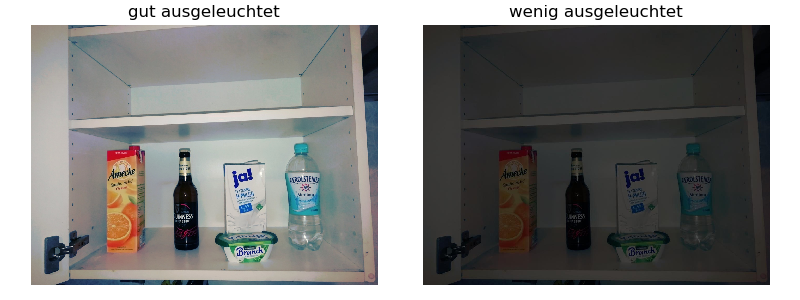
\includegraphics[scale=0.7]{Sources/Vergleich.png}
	\caption{Szene mit unterschiedlicher Ausleuchtung}
	\label{img:problem}
\end{figure}
\section{Erläuterung der These}\label{s.these}
Für solche Probleme bietet die Bildverarbeitung einige Lösungsansätze, welche theoretisch eine konstante Farbgebung und dadurch eine Erhöhung der Genauigkeit bringen könnten. Ob in der praktischen Ausführung die erwarteten Ergebnisse erzielt werden können, soll getestet werden. In dieser Arbeit sollen verschiedene Verfahren zur Farbnormalisierung von Bildern auf die Trainings- und Testdatensätze angewendet werden. Mit diesen normalisierten Datensätzen sollen daraufhin verschiedene künstliche neuronale Netze trainiert werden. Beim Vergleich der Trainingsergebnisse soll herausgestellt werden, ob das Normalisieren der Daten einen positiven Einfluss auf die Genauigkeit hat und welche Unterschiede die Normalisierungsverfahren aufweisen.
\section{Anforderungen}\label{s.anforderungen}
Bei dem geplanten Vorhaben, welches diese Arbeit thematisiert, ist es wichtig Anforderungen an das neuronale Netz, den Datensatz und die verwendeten Algorithmen zu formulieren, um sicher zu stellen, dass keine vermeidbaren Probleme auftreten. Zunächst werden Trainingsdaten benötigt, mit welchen die neuronalen Netze trainiert werden. Viele wissenschaftliche Arbeiten zeigen, dass eine große Menge an Daten benötigt wird, um ein gut funktionierendes neuronales Netz zu entwickeln. Im Schnitt werden 50.000 Trainingsbilder pro Klasse benötigt. Diese Menge an Daten kann in Anbetracht der verfügbaren Zeit nicht für drei verschiedene Datensätze generiert werden. Daraus ergbit sich folgende Anforderung:
\begin{enumerate} 
\item Die Menge an benötigten Trainingsdaten pro Klasse soll gering gehalten werden.
\end{enumerate}
Damit genügend Vergleichswerte untersucht werden können, sollen mehrere Datensätze mit unterschiedlichen Klassen genutzt werden. Um sicher zu stellen, dass die Datensätze für das Vorhaben geeignet sind, werden diese für die Arbeit erstellt und ausgesucht.\\\\
Die Trainingsdaten sollen unter folgenden Anforderungen erstellt werden:
\begin{enumerate} 
\setcounter{enumi}{1}
\item Ein qualitativ hochwertiger Datensatz sollte nicht unordentlich sein, da das Reinigen der Daten lange dauern kann. Das bedeutet, dass Klassen getrennt voneinander gespeichert werden, und die Namensgebung für jede Objektklasse klar definiert ist. Bei Problemfällen können Daten entfernt oder hinzugefügt werden.
\item Der Datensatz sollte Bilder enthalten, welche eine nicht zu hohe Auflösung besitzen, da sie den Trainingsfortschritt zurückhalten und mehr Ressourcen benötigen. Je größer das Bild ist, desto mehr Zeit wird für die Verarbeitung benötigt.
\item Beim Generieren der Trainingsbilder sollte darauf geachtet werden, saubere und gut ausgeleuchtete Aufnahmen zu machen. Aufnahmen der Objekte sollten nicht zu stark verschwimmen und unscharf werden. 
\item Das Ziel des Datensatzes sollte gut definiert werden. Namen und Thema des Datensatzes sollten auf einen gewissen Bereich beschränkt werden. Beispielsweise sollten keine Gesichter zusammen mit Pflanzen kombiniert werden. 
\end{enumerate}
Um die Auswirkungen der Normalisierungsverfahren vergleichen zu können, werden verschiedene Verfahren auf die selben Trainings- und Testdaten angewendet. Woraus sich folgende Anforderung ergibt:
\begin{enumerate} 
\setcounter{enumi}{5}
\item Anwendung der Normalisierungsverfahren auf verschiedene Datensätze
\end{enumerate}
  Durch die Normalisierungsverfahren soll die Farbvarianz verringert werden.
  \section{Struktur der Arbeit}\label{Struktur} 
Für ein besseres Verständnis der einzelnen Entwicklungsschritte in den späteren Kapiteln, werden in Abschnitt \ref{s.digibilder} zuerst die Grundlagen der digitalen Bildverarbeitung beschrieben. Dabei soll zunächst vermittelt werden, wie digitale Bilder entstehen und aus welchen Komponenten diese zusammengesetzt sind. Im Weiteren wird in Abschnitt \ref{s.neuronalenetze} auf die Funktionsweise künstlicher neuronaler Netze eingegangen. Hierbei werden die unterschiedlichen Schichten, welche durchlaufen werden, aufgeführt und beschrieben. Anschließend werden in Abschnitt \ref{s.nalgorithmen} die verwendeten Farbnormalisierungsverfahren erklärt und beschrieben. Der Ansatz der einzelnen Methoden wird erläutert, sowie auch die verwendeten Trainingsdaten und Modelle.\\\\
In der zweiten Hälfte der Arbeit wird es um die Durchführung und Ergebnisauswertung (Kapitel \ref{s.ergebnisse}) des praktischen Teils der Arbeit gehen. In diesem werden die verwendeten Farbnormalisierungsverfahren zusätzlich in der technischen Umsetzung erläutert. Daraufhin werden die Ergebnisse aufgeführt und interpretiert. In einer kurzen Diskussion (Kapitel \ref{s.diskussion}) werden diese behandelt. Nach der Diskussion wird nun das Ergebnis der Auswertung anhand der angeführten These evaluiert und ein Fazit (Kapitel \ref{s.fazit}) der Arbeit gezogen. 

	% Die Zähler für Tabellen und Abbildungen werden zurückgesetzt, damit
	% in jedem Kapitel die Nummerierung neu beginnt
\setcounter{table}{1}
\setcounter{figure}{1}
	% Einbinden des zweiten Kapitels
	%!TEX root = ../draft.tex
\chapter{Theoretische Grundlagen}\label{s.grundlagen}
Das folgende Kapitel soll eine kurze und leicht verständliche Einführung sein, in dem die theoretischen Grundlagen über den Aufbau von digitalen Bildern, den Einfluss von Belichtung sowie den verwendeten Bildbearbeitung Methoden gelegt werden. Anschließend folgt ein Überblick über die Grundlagen der künstlichen Intelligenz. Der letzte Abschnitt wittmed sich den Schwerpunkten der künstlichen neuronalen Netze. Dabei werden hauptsächlich für die Arbeit relevante Grundlagen vermittelt. 
\section{Digitale Bilder}\label{s.digibilder}
Damit der Ansatz der These, dass die Farbnormalisierung von Trainingsdaten das Trainingsverhalten und die spätere Genauigkeit künstlicher neuronaler Netze verbessern kann, nachvollzogen werden kann, soll in diesem Abschnitt, auf die Aufnahme digitaler Bilder, mit deren Eigenschaften und Aufbau eingegangen werden. Außerdem sollen die Schwächen herausgearbeitet und mögliche Lösungsansätze erläutert werden. Zunächst folgt eine kurze Einführung.\\\\
Bildverarbeitung, wird in der heutigen Zeit oft mit Bildbearbeitung assoziiert, also mit der Bearbeitung von Bildern mittels Bearbeitungssoftware. In der Bildverarbeitung geht es, anders als in der Bearbeitung, um die Software selber, welche für die Konzeption und Erstellung von digitalen Bildern genutzt wird. Die digitale Repräsentation eines aufgenommenen Bildes erfolgt als zweidimensionale Matrix, wie in Abbildung \ref{img:digitalesbild} zu erkennen, welche man nach Belieben lesen und verändern kann, um seine geplanten Ziele zu erreichen. Grundsätzlich bestehen digitale Bilder aus Rastern. Diese besitzen mehrere Werte, welche auch Pixel genannt werden. Die Werte entstehen je nach Menge der Farbabstufungen. Bei einem Graustufenbild sind das normalerweise 256 Abstufungen bei einem 8 bit Bild. 
\begin{figure}
[h]
\centering
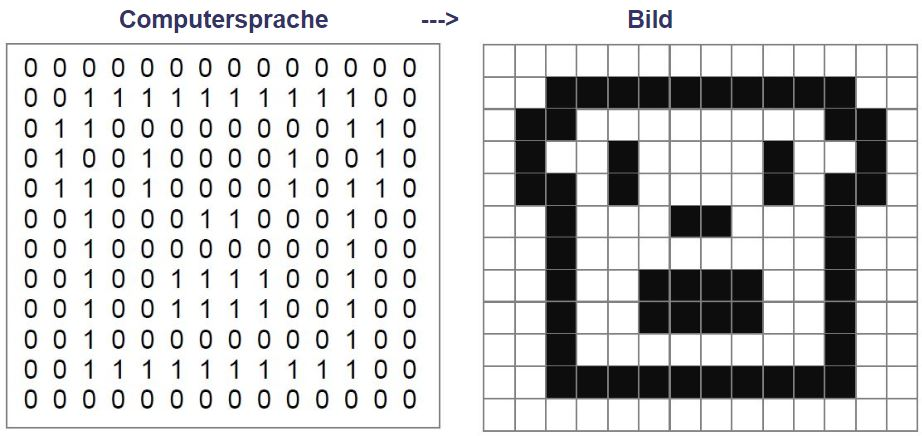
\includegraphics[scale=0.5]{Sources/Digitalesbild.JPG}
\caption{Aufbau eines Digitalen Bildes mit zwei Helligkeitsabstufungen}
\label{img:digitalesbild}
\end{figure}\\
In diesen Pixeln werden Bildinformationen wie Farbe und Position festgehalten. Jeder Pixel besteht dabei oft aus drei Kanälen, dem R Kanal für Rot, dem G Kanal für Grün und dem B Kanal für Blau. Diese bilden in bestimmten Kombinationen und Intensitäten ungefähr 16 Millionen verschiedene Farben. Der beschriebene Aufbau wird bei RGB-Bildern verwendet und auch bei Monitoren, Smartphones, etc. Neben dem RGB gibt es noch einige verschiedene Farbräume (RGB, HSV, CMY(K), YUV, etc).
\subsection{Farbräume digitaler Bilder}\label{s.aufbdigibilder}
Üblicherweise wird bei Digitalbildern mit dem RGB-Farbraum gearbeitet. Aus diesem Grund, wird in dieser Arbeit hauptsächlich auf RGB-Bilder eingegangen. Ein Bild ist wie eine Matrix aufgebaut, dabei kann es sowohl quadratisch wie auch rechteckige Abmessungen haben. Jeder Punkt in der Matrix stellt einen Pixel dar und enthält jeweils einen Rot-, Grün-, Blauwert welche zusammen eine beliebige Farbe darstellen. Um die Farbverteilung in einem Bild besser erkennen zu können, werden die Farbwerte in sogenannten Farb-Histogrammen zusammengefasst. Histogramme spielen für die Normalisierungsfunktionen eine Rolle. Aus diesem Grund wird das Konzept hinter den Histogrammen und die spätere Manipulation beschrieben. Einfachheitshalber werden Graustufenbildern für die Erklärung verwendet. Anwendbar sind diese auch auf die Histogramme der einzelnen RGB-Kanäle.\\\\
\textbf{RGB}\label{s.rgb}\\
Der RGB-Farbraum ist der geläufigste und bekannteste Farbraum dieser besteht, wie in Abschnitt \ref{s.digibilder} kurz beschrieben, aus drei Farbräumen (Rot-Grün-Blau). Dies beschreibt, welche Art von Licht ausgestrahlt werden muss, um eine gewünschte Farbe zu erreichen. Die Kombination der einzelnen Farbräume ist eine additive Farbmischung. RGB ist eher ein Farbmodell, da es viele Farbräume gibt, welche sich davon ableiten (sRGB, AdobeRGB, etc.).\\\\
\textbf{CMY(K)}\label{s.cmy}\\
Anders als der RGB-Farbraum benutzt der CMY-Farbraum den subtraktiven anstelle der additiven Farbmischung. Hierbei sind die drei Grundfarben C für Cyan, M für Magenta und Y für Yellow. Bekannt ist diese Farbmischung gerade durch das Malen von Wasserfarben, oder für die Farbpigmente, welche in Druckern genutzt werden. Für den durch die Farbmischung kann der CMY kein richtiges Schwarz erreichen, deswegen wurde der Farbraum CMYK mit einem Parameter erweitert. Das K steht für Schwarz, damit auch schwarz richtig dargestellt werden kann und kein dunkles Grau entsteht.\\\\
\textbf{HSV}\label{s.hsv}\\
Anders als der RGB ist der HSV-Farbraum aufgebaut. Dennoch gibt es auch hier drei Werte. Das H (Hue) steht für den Farbton, welcher angenommen werden soll, S (Saturation) für die Sättigung der ausgewählten Farbe und V (Value) für den Helligkeitswert oder auch die Helligkeit der Farbe. Dieser Farbraum ist gerade in der Kunst beliebt, da die Farbvorstellung besser funktioniert als bei additiven und subtraktiven Farbmischungen. Denn beim malen wird mit Farben gearbeitet, in welchen lediglich die Sättigung sowie die Helligkeit verändert wird.\\\\
\textbf{YUV}\label{s.lab}\\
Das YUV-Farbmodell, wird hauptsächlich beim analogen Fernsehen verwendet. Dieser Farbraum verwendet zur Darstellung von Farben zwei Komponenten. Die Lichtstärke oder auch Luminanz (Y) genannt, sowie die Chrominanz (Farbanteil) welche wiederum aus den zwei Unterkomponenten U und V besteht. U und V geben somit die Farbe an. Dafür werden U und V in ein vierteiliges Koordinatensystem gelegt. Auf der X-Achse liegt V und auf der Y-Achse U, dabei besitzt jedes Feld des Koordinatensystems eine Farbe (Rot, Violett, Blau und Grün). Die Farbe wird durch die Kombination beider Werte (U und V) bestimmt. Y stellt das Helligkeitssignal in dem Farbraum dar und gibt an wie hell die Farbe dargestellt werden soll. Anders als beim HSV-Farbraum wird die Lichtstärke und Sättigung der Farbe durch einen Kanal bestimmt. 
\subsection{Histogramme}\label{s.histogramme}
Histogramme beschreiben eine Häufigkeitsverteilung \cite[42ff.]{burger2009digitale}. Speziell bei Bildern zeigen Histogramme die Häufigkeit der auftretenden Intensitätswerte. Am einfachsten lässt sich das mit Graustufenbildern nachvollziehen. Ein Beispiel dafür zeigt die (Abbildung \ref{img:histogramm}) für ein Graustufenbild $I$ mit möglichen Intensitätswerten im Bereich $I(n,V)E[0,K-1]$ enthält das Histogramm $H$ genau $K$ Einträge. Die Menge der Einträge bei einem 8 Bit Graustufenbild sind $2^8$ Farbabstufungen ($K=2^8=256$). Der Wert des Histogramms an der Stelle $i$ ist $h(i)$ die Anzahl der Pixel von $I$ mit einem Intensitätswert $i$, für alle ($0<i<K$). Mathematisch ausgedrückt ergibt sich $h(i)=card{(u,v) | I(u,v)=i}$\\
  daraus lässt sich entnehmen, dass $h(0)$ die Anzahl der Pixel mit dem Wert 0, $h(1)$ die Anzahl des Wertes 1 usw., $h(255)$ ist schließlich der letzte Wert und gibt die Menge aller weißen Pixel in dem Bild an $(K-1)$. Eine Histogramm-Berechnung stellt somit einen eindimensionalen Vektor $h$ der Länge $K$ dar.\\
  \begin{figure}
    [h]
    \centering
    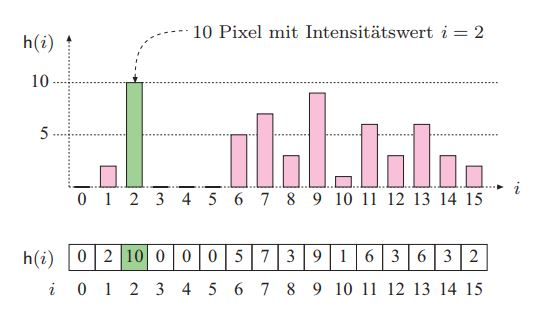
\includegraphics[scale=0.8]{Sources/histogramm.jpg}
    \caption{Histogramm eines Graustufen-Bildes mit 16 Helligkeitsabstufungen \cite[42]{burger2009digitale}}
    \label{img:histogramm}
  \end{figure}
$card$ beinhaltet die Anzahl der Elemente einer Menge (\textit{Kardinalität})\\\\
Die Abbildung \ref{img:histogramm} zeigt ein mögliches Histogramm mit einer Farbabstufung von 16 Werten. Ein Histogramm zeigt die wichtigsten Eigenschaften eines Bildes, wie beispielsweise die Dynamik oder den Kontrast eines Bildes. Außerdem lässt sich erkennen, ob bei der Bildaufnahme Probleme aufgetreten sind. Diese lassen sich erkennen, indem Ausschläge ganz links oder ganz rechts, des Graphen zu erkennen sind. Ein Ausschlag bei 0 oder 255 bedeutet das dort keine Farbinformationen mehr vorhanden sind und, dass Teile des Bildes, über- beziehungsweise unterbelichtet sind.\\\\
\textbf{Kontrast}\label{s.kontrast}
Der Kontrast bezeichnet den Bereich von Intensitätstufen, welche in einem Bild effektiv genutzt werden, also die Differenz der maximalen und minimalen Pixelwerten \cite[44]{burger2009digitale}. Ein Bild, welches einen hohen Kontrast hat, nutzt das gesamte Spektrum des Histogramms (Schwarz bis Weiß). Der Kontrast lässt sich also leicht aus einem Histogramm entnehmen, wie in Abbildung \ref{img:dynamik} die verschiedenen Histogramme zeigen.\\\\
  \begin{figure}
    [h]
    \centering
    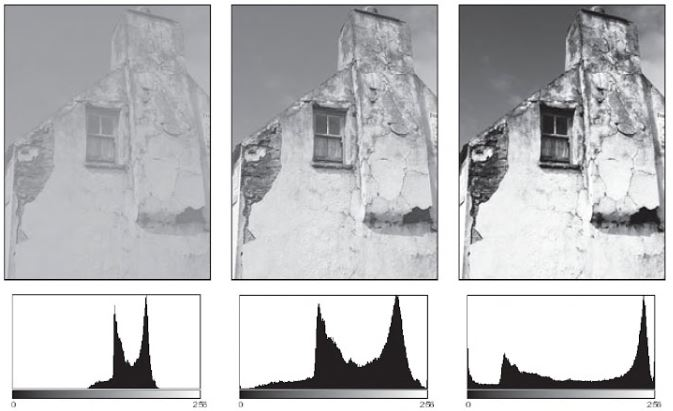
\includegraphics[scale=0.7]{Sources/kontrast.JPG}
    \caption{Unterschiedlicher Kontrast und die Auswirkungen im Histogramm: niedriger Kontrast (links), normaler Kontast (Mitte), hoher Kontrast (rechts)\cite[45]{burger2009digitale}}
    \label{img:kontrast}
  \end{figure}\\\\
\textbf{Dynamik}\label{s.dynamik}\\
Dynamik bedeutet, wie viel verschiedene Intensitätswerte in einem Bild genutzt werden, und die jeweilige Anzahl\cite[44]{burger2009digitale}. Im besten Fall entspricht die Dynamik der insgesamt genutzten Anzahl an Pixelwerten (Abbildung \ref{img:dynamik}). Also $K-1$ genutzter Farbabstufungen, damit der Wertebereich voll ausgeschöpft wird.\\
 \begin{figure}
    [h]
    \centering
    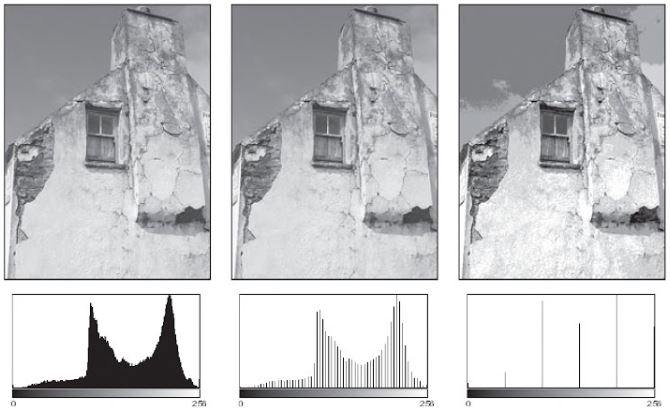
\includegraphics[scale=0.7]{Sources/dynamik.JPG}
    \caption{Unterschiedlicher Dynamik und die Auswirkungen im Histogramm: hohe Dynamik (links), niedrige Dynamik mit 64 Graustufen (Mitte), extrem niedriger Kontrast mir 6 Graustufen (rechts)\cite[45]{burger2009digitale}}
    \label{img:dynamik}
  \end{figure}\\
Anders als der Kontrast, welcher immer erhöht werden kann, solange der maximale Wertebereich nicht erreicht worden ist, kann die Dynamik eines Bildes nicht so leicht verbessert werden. Aus diesem Grund ist eine hohe Dynamik von Vorteil. Denn dadurch wird die Gefahr von Qualitätsverlust bei Verarbeitungsschritten verringert. Trotz der Tatsache, dass viele Ausgabegeräte mit Farbtiefen von 8 Bit arbeiten, nehmen heutige Kameras bis zu 12-14 Bit pro Kanal auf, um einem möglichen Qualitätsverlust vorzubeugen.
\subsection{Einfluss von Belichtungen}\label{s.belichtung}
In dem Kapitel \ref{s.aufbdigibilder} wurde beschrieben, wie die Farben in Bildern gespeichert werden und welche unterschiedlichen Arten von Farbräumen es gibt \cite[41ff.]{burger2009digitale}. Bei der Aufnahme von Bildern ist gerade die Belichtung entscheidend. Eine hohe Belichtung sorgt dafür, dass Farben heller wirken, wobei wenig Licht dafür sorgt, dass Farben dunkler erscheinen. Diese Tatsache kann beim Deep Learning zu Problemen führen, da ein und dasselbe Objekt unterschiedliche Farben annehmen kann und je nach Belichtungsintensität variiert. Ein künstliches neuronales Netz kann Objekte, welche es normalerweise trainiert hat, nicht immer erkennen, wenn die Farbe zu stark von der eigentlichen Farbe abweicht. Um Belichtungen auf Bildern auszugleichen und zu normalisieren, gibt es einige Verfahren, welche diesem Problem entgegenwirken. Die ausgewählten Verfahren werden aufgeführt und beschrieben. Diese stellen nicht die Originalfarbe des Objektes wieder her, sondern sorgen für eine konstante Farbvariation, welche sich nicht stark verändert.
\section{Künstliche Intelligenz}\label{s.ki}
In den letzten Jahren hat die Nutzung von künstlichen Intelligenzen enorm zugenommen und Firmen nutzen diese Technologie beispielsweise für die Analyse und Vorhersage von Kundenverhalten, für die Klassifikation von Bildern oder zur Spracherkennung in heutigen Smartphones. Mit künstlicher Intelligenz beschreibt man solche Computer, welche gewisse Aufgaben erledigen, ohne ausdrücklich dafür programmiert worden zu sein. Dabei werden Informationen anhand von Vergleichsdaten dem System zugeführt, wodurch er sich Eigenschaften und Strukturen merkt und durch diese Rückschlüsse und Prognosen ziehen kann. Eine gute Beschreibung geben dabei die Autoren Rich und Knight, indem sie schrieben:\\\\
 \textit{Das Studium des Problems, Computer dazu zu bringen, Dinge zu tun, bei denen ihnen momentan der Mensch noch überlegen ist.} - (Rich und Knight 1991)\\\\
Ein gutes Beispiel in welchem man das Potenzial von künstlicher Intelligenz sehen kann, ist die Spiele-KI  \textit{AlphaGo}. Diese KI wurde von Google entwickelt und ist auf das Spielen des Brettspiels Go trainiert. So konnte \textit{AlphaGo} in einem Match 2016, den damaligen Weltmeister in Go \textit{Lee Sedol} schlagen \cite{Alpha2016GO}. In vier von fünf Spielen gewann der Computer. Solche Ergebnisse konnten bis zu diesem Zeitpunkt mit anderen Methoden nicht erzielt werden, da es für damalige Algorithmen zu viele mögliche Spielzüge gab. Durch Deep Learning konnte der Computer ohne feste Algorithmen, besser als der Weltmeister, seine Spielzüge planen. Anhand der Definition von Rich kann man feststellen, dass  \textit{AlphaGo}  im Bereich des Spieles Go als intelligent zählt, da sie dem besten Go-Spieler der Welt deutlich überlegen war.
  \section{Neuronale Netze}\label{s.neuronalenetze}
Um das Konzept hinter den künstlichen neuronalen Netzen besser verstehen zu können, betrachten wir zunächst, wie der Lernprozess eines Menschen abläuft. Menschliches Lernen ist das Verändern der eigenen Verhaltensstrukturen und die Folgen individueller Erfahrungen \cite{hoffmann2016lern}. Der Lernprozess, kann sowohl bewusst sowie auch unbewusst unser Verhalten verändern. Menschen adaptieren also die eigenen als auch fremde Erfahrungen zu ihren Gewohnheiten. Diese Prozesse finden im Gehirn statt, welches aus vielen Nervenzellen besteht. Diese Nervenzellen werden Neuronen genannt und sind untereinander verknüpft, weshalb auch von einem neuronalen Netz gesprochen wird. Maschinelles Lernen nimmt sich also die Funktionsweise des menschlichen Gehirns zum Vorbild \cite[]{ertel2013grundkurs}.\\\\
\textbf{Menschliches Lernen}\\
Wie bereits erwähnt, sind der Aufbau sowie die Funktionsweise von künstlichen neuronalen Netzen vom menschlichen Gehirn abgeleitet. Das Gehirn besteht aus ungefähr $10^{11}$ Nervenzellen, welche untereinander verknüpft sind \cite[265ff.]{ertel2013grundkurs}. Für den Lernprozess sind demnach viele Neuronen nötig. In der Abbildung \ref{img:neuron} kann man den wesentlichen Aufbau eines Neurons sehen.
\begin{figure}
	[h]
	\centering
	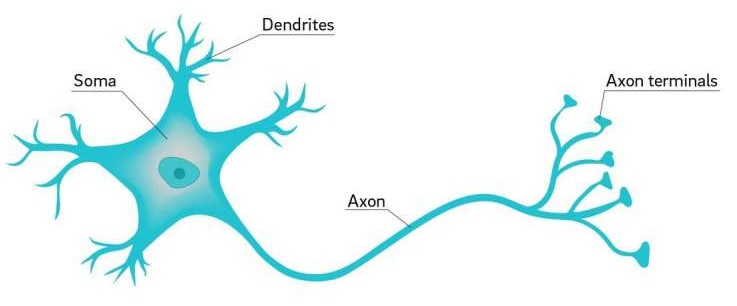
\includegraphics[scale=0.7]{Sources/neuron.jpg}
	\caption{Aufbau eines Neurons \cite{neuron2018UoC}}
	\label{img:neuron}
\end{figure}\\
In diesem vereinfachten Modell eines Neurons lassen sich die wesentlichen Komponenten erkennen. Das Neuron selber besteht aus einem Zellkörper (Soma), einem Axon, den Dendriten auf der linken Seite und den Synapsen(Axon Terminals) auf der rechten Seite. Eine Dendrite stellt mit der Synapse eine Verbindung zu anderen Neuronen her. Diese senden elektrische Impulse an die Soma weiter, welche verarbeitet werden. Wenn die Spannung einen gewissen Schwellwert übersteigt, sendet die Soma einen elektrischen Impuls über das Axon. Jede Synapse sendet das Signal an die Dendriten des nächsten Neurons weiter. Die Stärke des Impulses und der Schwellwert, ist bei jedem Neuron unterschiedlich und verändern sich ständig. Der Schwellwert des Neurons ist niedriger, desto öfter es aktiv ist und steigt wenn es selten aktiv ist \cite{schmidt2013physiologie}. Die aufgeführte Funktionsweise beschreibt nur oberflächlich das Verhalten eines neuronalen Netzes und soll hauptsächlich dem weiteren Verständnis dienen.\\\\
\textbf{Perzeptron}\\
Die Grundlage für den mathematischen Ablauf künstlicher neuronaler Netze wurde von McCulloch und Pitts in ihrem Buch \textit{A logical calculus oft he ideas immanent in nervous activity} erklärt. Auf diesen Grundlagen simulierte 1953 der Psychologe und Informatiker Frank Rosenblatt das erste künstliche Neuron, welches auch als Perzeptron bekannt wurde. In der Abbildung \ref{img:Perzeptron} wird der Aufbau eines solchen Perzeptrons dargestellt.\\\\\\\\
\begin{figure}
	[h]
	\centering
	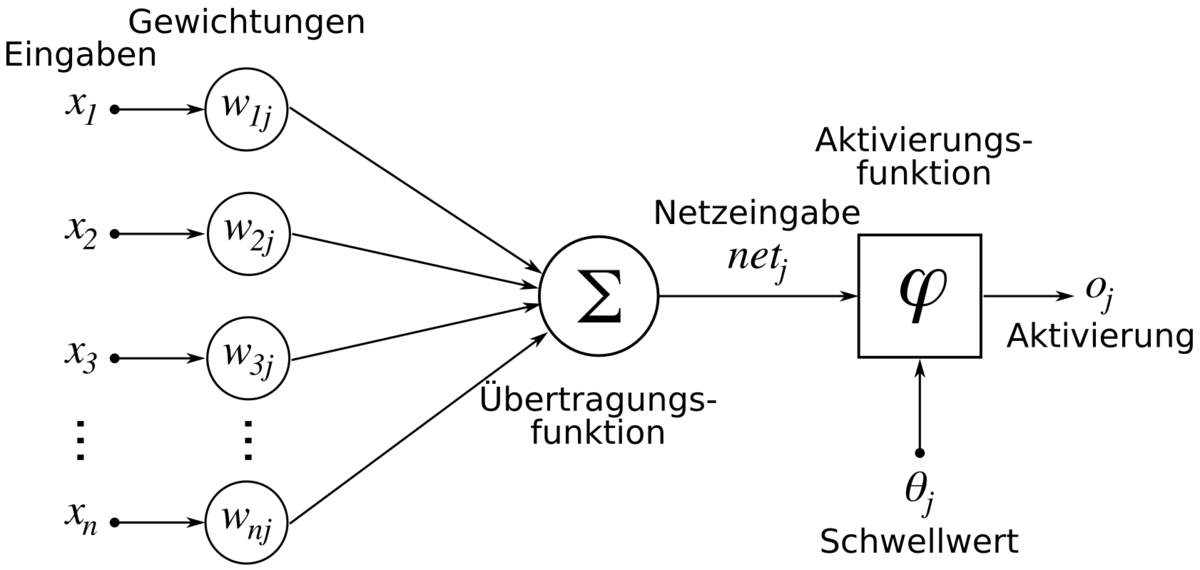
\includegraphics[scale=0.3]{Sources/perzeptron2.png}
	\caption{Schematische Modellierung eines Perzeptrons nach Rosenblatt \cite{perzeptron2019}}
	\label{img:Perzeptron}
\end{figure}\\
Als Eingabewert bekommt das Perzeptron ein Gewicht $w$, welches mit den Eingangswert $x$ multipliziert wird. Das Ergebnis dieser beiden Werte, kann als lineare Funktion beschrieben werden.
\begin{eqnarray} f(x) & = & w*x \end{eqnarray}
Das Ergebnis der beiden Werte wird an eine Aktivierungsfunktion $g$ übergeben. Die Aktivierungsfunktion oder auch Schwellwert genannt, gibt ein Signal weiter, sobald dieser Wert überschritten wird.
\begin{eqnarray} g( \sum_{i=0}^n x_{i} *w_{i}) \end{eqnarray}
Als Aktivierungsfunktion können sowohl lineare als auch nicht linearen Funktionen verwendet werden. Zusätzlich wird dem Ergebnis der Funktion der \textit{Bias} $b$ addiert.
\begin{eqnarray} g(( \sum_{i=0}^n x_{i} *w_{i}) +b \end{eqnarray}
Der \textit{Bias} ist eine Art zusätzliches Neuron, für das Verringern von Konvergenz-Problemen, welche bei der Approximation der Funktion auftreten können. Der Bias hat immer einen Eingabewert von 1 und ein Gewicht $w_{jb}$, welches unabhängig der Eingabewerte ist.
\begin{eqnarray} Bias = 1*w_{jb} \end{eqnarray}
Maschinelles Lernen möchte unter anderem Maschinen in die Lage versetzten Objekte, Strukturen oder auch Abläufe anhand von vorher beigebrachten Beispielen eigenständig zu erkennen. Eine Methode, um dieses Ziel erreichen zu können sind die künstlichen neuronalen Netze. Diese werden mit Datensätzen des jeweiligen Schwerpunktes trainiert. Es gibt vier grundlegende Methoden ein solches Netz zu trainieren.\\\\
\textbf{Überwachtes Lernen}\\
Das überwachte Lernen funktioniert hauptsächlich mit Datensätzen, welche Eingabedaten sowie Ausgabedaten enthalten. Das künstliche neuronale Netz versucht bei Eingabe der Daten, eine Funktion aufzustellen, welche eine Hypothese darstellt. Diese beschreibt um, was es sich bei dem Datensatz handelt. Die Genauigkeit dieser Hypothese kann durch den Vergleich der enthaltenden Ausgabedaten ermittelt werden. Wenn die Möglichkeiten der Ausgaben endlich sind, handelt es sich um eine Klassifizierung (Bsp.: Milch, Orangensaft, Wasser, etc.). Sollten nur zwei Ausgabewerte möglich sein, ist es eine boolsche bzw. binäre Klassifizierung. Eine Zahl als Ausgabe wird als Regression bezeichnet.\\\\
\textbf{Nicht überwachtes Lernen}\\
Die zweite Methode, wie ein künstliches neuronales Netz trainiert werden kann, ist eine gegenteilige Herangehensweise. Hier werden lediglich die Eingabedaten übergeben. Das neuronale Netz versucht selbstständig auftretende Muster in den Daten zu erkennen. Als Beispiel könnte man die sinnvolle Zuordnung von Bildern anhand ähnlicher Muster nehmen. Ähnliche Datensätze werden in Kategorien aufgeteilt, jedoch nicht benannt.\\\\
\textbf{Halb überwachtes Lernen}\\
Oft werden die beiden Methoden des überwachten und unüberwachten Lernen kombiniert. So hat man meist einen kleinen Datensatz mit Ein- und Ausgabedaten, welche aber nicht explizit wahr sein müssen und einen Teil nur mit Eingabeinformationen. Diese Methode wird häufig bei Umfragen verwendet, wo nicht klar ist, ob der Proband wahrheitsgemäß antwortet. Dabei kann ein systematischer Fehler entstehen. Daraus ergibt sich eine Mischung aus überwachtem Lernen mit systematischen Fehler und unüberwachtem Lernen, bei welchem das Netz nach häufig auftretenden Mustern sucht.\\\\
\textbf{bestärkendes Lernen}\\ 
Das verstärkte Lernen arbeitet auf einem Prinzip, mit welchem richtige Entscheidungen belohnt und falsche bestraft werden. Ein bekanntes Beispiel ist ein Netz, welches virtuell eine Rennstrecke ohne Fehler (nicht von der Strecke abkommen) beenden muss. Bei jedem Fehler muss von vorne begonnen werden, bis die Strecke beendet wird. Ein besonders bekanntes Beispiel ist die Go-KI \textit{AlphaGo} \cite{Alpha2016GO}, welche nur durch die Informationen der Spielregeln trainiert wurde.\\\\\\\\
\textbf{Künstliche neuronale Netze}\\
Nachdem etwas auf die Grundlagen der verschiedenen Lernverfahren eingegangen wurde, soll in diesem Abschnitt der Aufbau künstlicher neuronaler Netzes und die Logik fokussiert werden. Der mathematische Ablauf der Schichten wird in einem späteren Unterkapitel behandelt.\\
\begin{figure}
	[h]
	\centering
	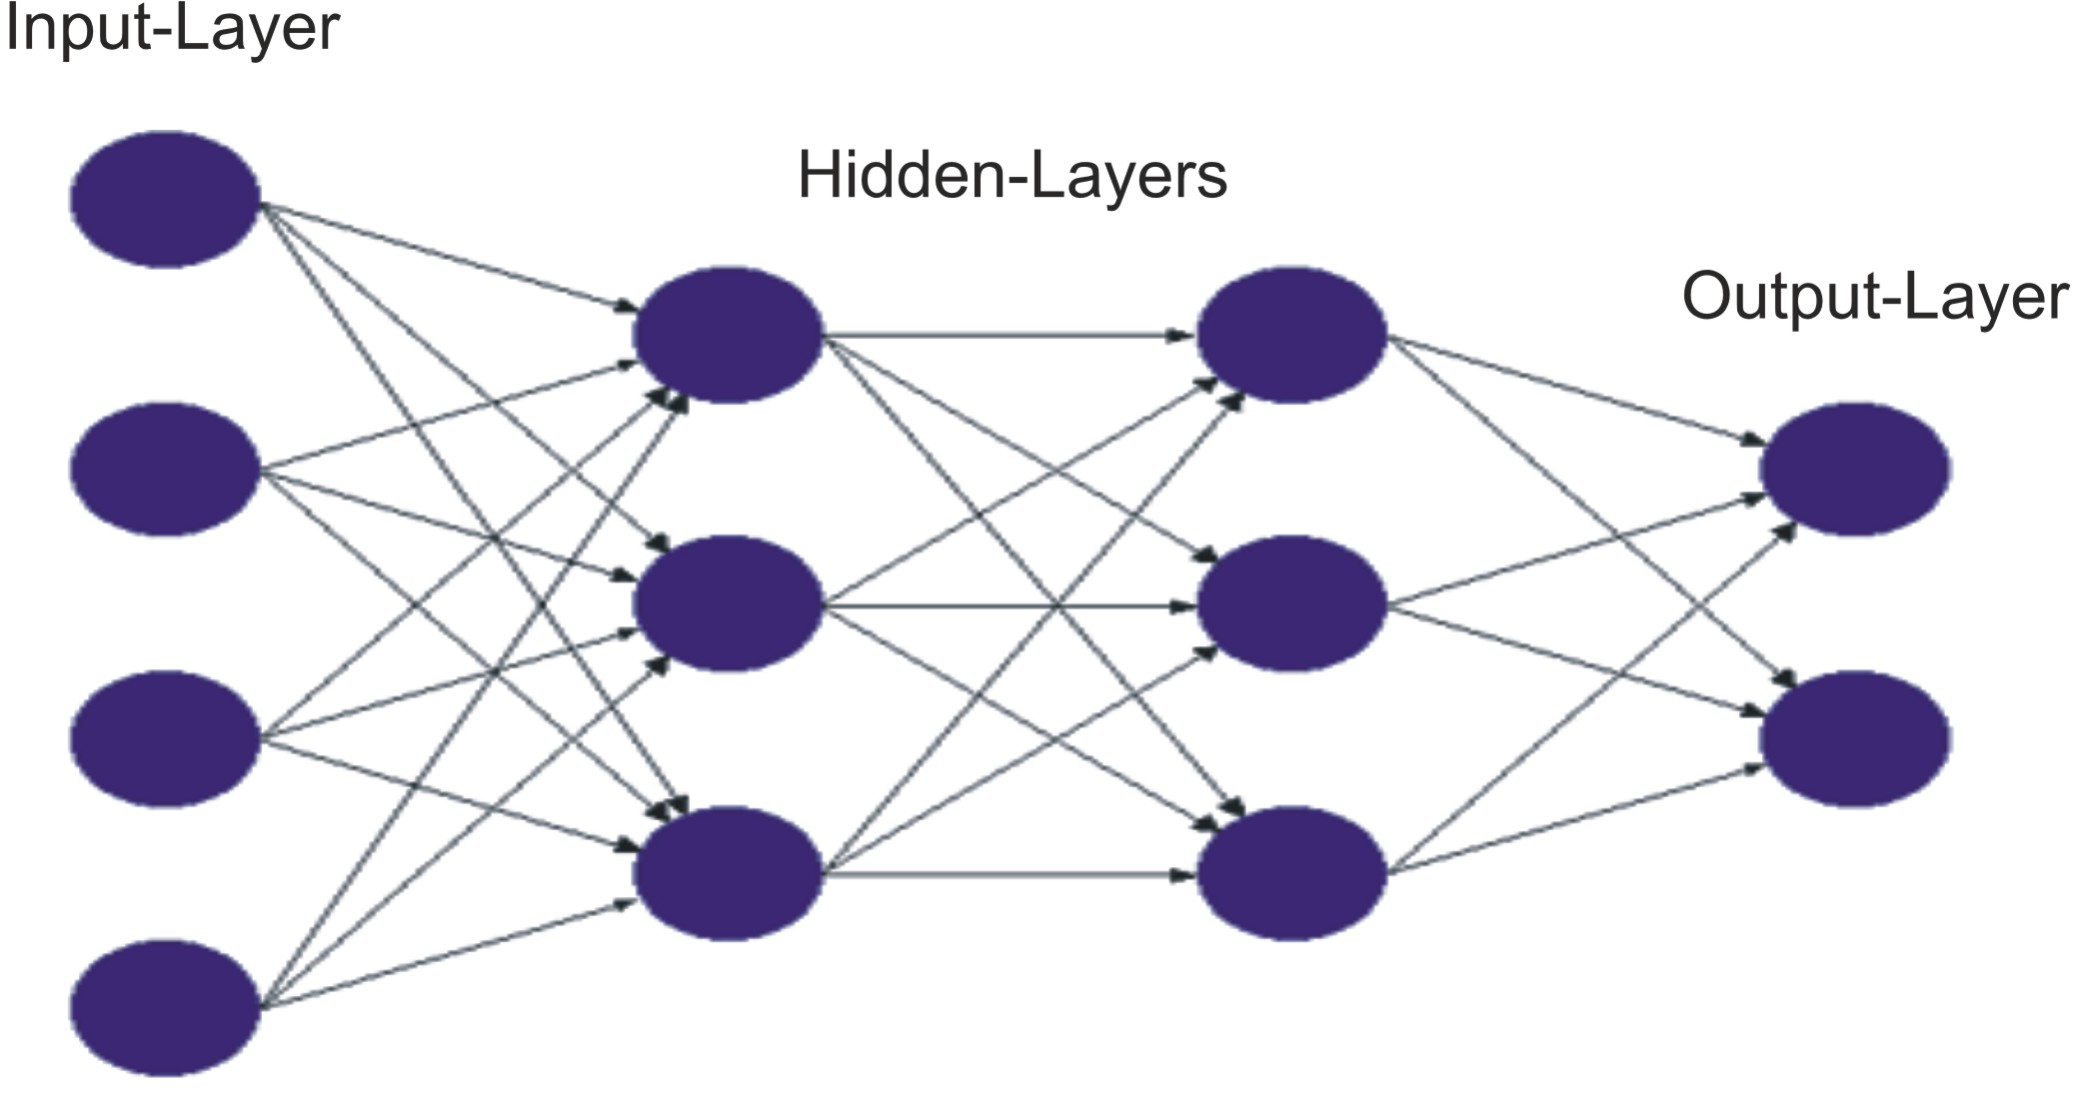
\includegraphics[scale=0.5]{Sources/nnet.png}
	\caption{Aufbau eines künstlichen neuronalen Netzes \cite{bistra2018pic}}
	\label{img:neuronales_netz}
\end{figure}\\
Der Aufbau von klassischen künstlichen neuronalen Netzen kann grundsätzlich in drei Bereiche unterteilt werden. Die erste Schicht stellt der \textit{Input Layer} dar. Dieser besteht, wie alle folgenden Schichten, aus mehreren Neuronen. In diese Schicht werden die Trainingsdaten eingegeben. Jeder Wert eines Datensatzes wird mit einem Neuron verbunden. Die Neuronen besitzen eine Gewichtung und einen Schwellwert. Wenn der Schwellwert durch den Eingabewert erreicht wird, sendet das Neuron das Ergebnis seiner Berechnungen an das Neuron der nächsten Schicht weiter. Die folgenden Schichten werden \textit{Hidden Layer} genannt. Die Anzahl der \textit{Hidden Layer} ist variabel und kann so viele Schichten enthalten, wie benötigt. Diese Schichten werden auf mehrere verschiedene Merkmale der Eingabedaten trainiert. Dabei werden in frühen Schichten zunächst grobe Strukturen erkannt, welche nach jeder Schicht immer feiner werden. Die letzte Schicht des \textit{Hidden Layer} übergibt seine Informationen an den \textit{Output Layer}. Dieser stellt durch die erhaltenen Daten eine Hypothese auf, in welcher er beschreibt, wie er den Datensatz zuordnet. Dabei gibt das Netz an, zu welcher Wahrscheinlichkeit die Hypothese richtig sein sollte.\\\\
\textbf{Faltende neuronale Netze}\label{s.cnn}\\
\textit{Convolutional neural Networks} oder auch faltende neuronale Netze (Abbildung \ref{img:cnn}) sind, anders als das künstliche neuronale Netz, an das Konzept des menschlichen Sehens angelehnt \cite{sermanet2012convolutional} und für das Verarbeiten von matrixartigen Datensätzen konzipiert. Dazu zählen beispielsweise Bildaufnahmen \cite{goodfellow2016deep}. Die erste Schicht besteht aus dem \textit{Convolutional Layer}. Bei dieser Schicht wird über die Pixel des Eingabebildes eine Schablone gelegt und vertikal wie auch horizontal verschoben. Diese Schablone hat eine ungerade quadratische Abmessung ($3x3$, $5x5$, $7x7$) und eigene Gewichtungen. Diese Schablone bildet ein Skalarprodukt der unterliegenden Pixel und der Gewichtung. Dabei werden die Strukturen hervorgehoben. Diese Schicht kommt mehrmals in einem Netz vor.\\  
\begin{figure}
	[h]
	\centering
	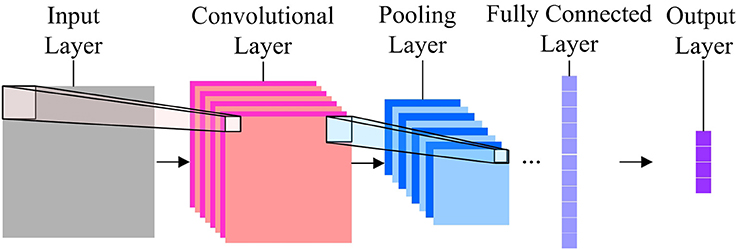
\includegraphics[scale=0.5]{Sources/cnnet.jpg}
	\caption{Aufbau eines Convolutional neural Network \cite{info7040061}}
	\label{img:cnn}
\end{figure}\\
Auf den \textit{Convolutional Layer} folgt immer der \textit{Pooling Layer}. Dieser ist für die Komprimierung des Eingabebildes zuständig, damit im späteren Verlauf Rechenleistung gespart werden kann. Auch diese Schicht besteht aus einer Schablone, welche über die Pixel des Bildes gelegt werden. Hierbei werden die Farbwerte der unterliegenden Pixel verarbeitet. Diese werden zu einem Wert zusammengefasst und übergeben. Nachdem alle \textit{Convolutional} und \textit{Pooling Layer} durchlaufen wurden, werden die Daten an die letzte Schicht (\textit{Fully Connected Layer}) übergeben. Der \textit{Fully Connected Layer} besteht wie beim KNN beschrieben, aus mehreren Perzeptronen-Schichten und gibt die Informationen an den \textit{Output Layer} weiter, welcher schlussendlich eine Hypothese mit zugehöriger Wahrscheinlichkeit ausgibt.\\\\
\textbf{Loss Funktion}\\
Bei jedem Trainingsschritt versucht das neuronale Netz, eine Hypothese aufzustellen. Damit das Netz Fortschritte im Lernen macht, ist das sogenannte Backpropagation, welches im nächsten Abschnitt genauer beschrieben wird, zuständig, welches auf der Basis des Loss Graphen arbeitet. Die Loss Funktion berechnet den Fehler, welchen das Netz in seinem aktuellen Zustand in der Berechnung begeht, also die Differenz zwischen dem Ist und Sollwert der Ausgabe. Beispiel einer solchen Funktion ist die euklidische Loss-Funktion:
\begin{eqnarray} E_{Euclid}&=&\frac{1}{2N} \sum_{n=1}^N || \hat{f_{n}}-f_{n} || \binom{2}{2} \end{eqnarray}
dabei stellt\\

	$\hat{f}_{n}[-\infty,+\infty]$ den berechneten Ist-Wert und
	
	$f_{n}$ den Sollwert dar\\\\
Das Ergebnis der euklidischen Funktion ist das Maß für den Grad der Abweichung von ist und Sollwert.\\\\
\textbf{Rückpropagierung}\\
Die Rückpropagierung oder auch \textit{Backpropagation} \cite{ertel2013grundkurs} ist unter anderem Teil des überwachten Lernens und beinhaltet das Lernen aus Fehlern. Dadurch, dass bei einer Klassifizierung Datensätze mit einem Zielwert verwendet werden, kann das Netz bei einer Zuweisung überprüfen, ob das Ergebnis zu dem Zielwert passt. Dabei wird aus der Ausgabe und dem Zielwert ein Fehler (Loss) berechnet. Sollte das Ergebnis zu weit vom Zielwert abweichen, wird überprüft, welches Perzeptron den größten Einfluss auf die Fehlzuweisung verursacht hat. Dieses Perzeptron wird in seiner Gewichtung angepasst, um den Fehlerwert zu verringern \cite{goodfellow2016deep}.  
  \subsubsection{Funktionsweise künstlicher und faltender neuronaler Netze}\label{s.funktwknnundcnn}
Die zuvor aufgeführten Netzarten haben einen unterschiedlichen Aufbau und bestimmte Einsatzgebiete. Das Convolutional neural Network ist beispielsweise auf das Verarbeiten von Bilddaten optimiert und Künstliche neuronale Netze eher für serielle Daten. In der Struktur sind die Netzarten ähnlich aufgebaut. Das \textit{Convolutional neural Network} hat neben den üblichen Neuronenschichten zwei zusätzliche Schichten, welche beim künstlichen neuronalen Netz nicht vorhanden sind. In den folgenden Absätzen soll die Funktionsweise dieser zusätzlichen Schichten beschrieben werden.\\\\
\textbf{Faltungsschicht}\\
Es existieren eine Menge von Filtern $n$, welche eine Höhe von $f_{h}$ und eine Breite von $f_{w}$ haben. Diese Filter werden über das Eingabebild mit der Höhe $e_{h}$ und der breite $e_{w}$ gelegt und in ein Pixel schritten bewegt. Die Ergebnisse stellen eine Liste von Merkmalen dar, welche auf der Höhe $m_{h}$ und der Breite $m_{w}$ liegen. Formell ausgedrückt:
\begin{eqnarray} 
m_{h}&=&(e_{h} - f_{h})+1\\
m_{w}&=&(e_{w} - f_{w})+1
\end{eqnarray}
Um die Verringerung von Informationen nach der Faltung zu verhindern, werden an den Rändern der Bilder Polsterungen, auch \textit{padding} genannt, angehangen \cite[343]{goodfellow2016deep}. Diese Polsterungen bestehen aus Pixeln mit einem Wert von \textit{0}. Die Anzahl der zusätzlichen Pixel ergibt sich aus der Höhe und Breite des Eingabebildes, um wie viele Pixel das Bild vergrößert wird. Formell ausgedrückt:
\begin{eqnarray}
p_{h}&=&f_{h} - 1\\
p_{w}&=&f_{w} - 1
\end{eqnarray}
Die Faltungsschicht hat eigene Gewichte, welche beim Vorgang mit denen des Bildes zusammengerechnet werden \cite[331ff.]{goodfellow2016deep}. Für die gleiche Schicht wird derselbe Filter verwendet. Die Weise der Berechnung wird in der Abbildung \ref{img:faltungsschicht}  beschrieben.
\begin{figure}
	[h]
	\centering
	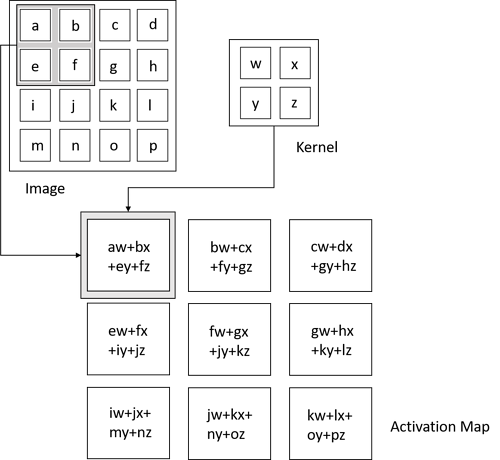
\includegraphics[scale=0.4]{Sources/CNN.png}
	\caption{Funktionsweise der Faltungsschicht \cite{convolutional2019layer}}
	\label{img:faltungsschicht}
\end{figure}\\
\textbf{Pooling Schicht}\\
Die Pooling Schicht oder auch \textit{Pooling Layer} kommt nach jeder Faltungsschicht \cite[336f.]{goodfellow2016deep}. Die Aufgabe dieser Schicht ist es, das Eingabebild in der Auflösung und den zugehörigen Rechenaufwand für die folgenden Schichten zu reduzieren. Üblicherweise gibt es zwei Verfahren, welche beim Pooling eingesetzt werden. Zum einen das Average Pooling und das am häufigsten verwendete Max Pooling (Abbildung \ref{img:maxpooling}). Auch diese Schicht besteht aus einem quadratischen Filter, welcher wie bei der Faltungsschicht über die Bildpunkte gelegt wird. Dabei wird beim \textit{Max Pooling} der höchste Wert in diesem Bereich ermittelt und übernommen. Bei einem standardmäßigem Kernel von 2x2, wird das Bild um den Faktor 2 verkleinert. Die Abmessungen sind, anders als bei der Faltungsschicht, gerade.
\begin{figure}
	[h]
	\centering
	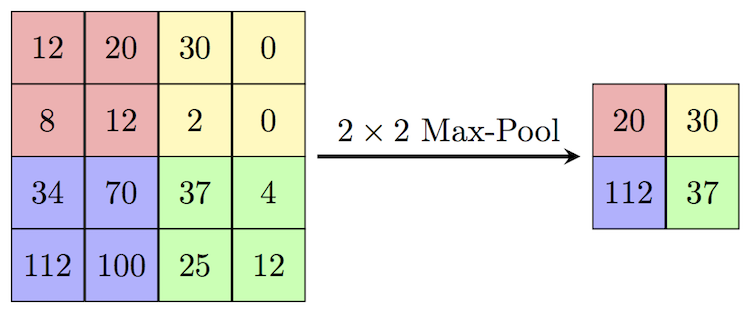
\includegraphics[scale=1.8]{Sources/MaxpoolSample2.png}
	\caption{Funktionsweise des Pooling Layers mit der Max Pooling-Variante \cite{pooling2018layer}}
	\label{img:maxpooling}
\end{figure}\\
\textbf{Fully connected Layer}\\
Nachdem das Eingabebild durch alle Faltungs- und Pooling Schichten verarbeitet wurde, werden die Daten an den Fully connected Layer übergeben \cite[14]{sermanet2012convolutional}. Dieser verwendet, wie bei einem normalen KNN, Perzeproten um die Daten zu verarbeiten. Die vorherigen Schichten wurden durchlaufen, damit diese rechenintensive Schicht nicht zu viele Informationen verarbeiten muss. 
  \subsection{Entstehung von Trainingsdaten}\label{s.trainingsdaten} 
Damit ein künstliches neuronales Netz Objekte erkennen und zuordnen kann, benötigt es zunächst eine Reihe von Beispieldaten. Anhand dieser Beispieldaten lernt das neuronale Netz, welche Eigenschaften das zu erlernende Objekt hat und wie es aufgebaut ist. Für diesen Vorgang werden üblicherweise mehrere hunderttausend Daten benötigt, um ein akzeptables Ergebnis zu erzielen. Eine Möglichkeit, das Training mit weniger Trainingsdaten durchzuführen, ist das Verwenden vortrainierter Netze. Diese Netze wurden mit rund 300.000 Bildern über mehrere Tage trainiert und als Open Source zur Verfügung gestellt. Beim Verwenden dieser Netze werden lediglich die obersten Schichten, welche für die Zuweisung verantwortlich sind, durch den neuen Datensatz verändert wodurch wesentlich weniger Testdaten pro Objektklasse benötigt werden. 
\begin{figure}
	[h]
	\centering
	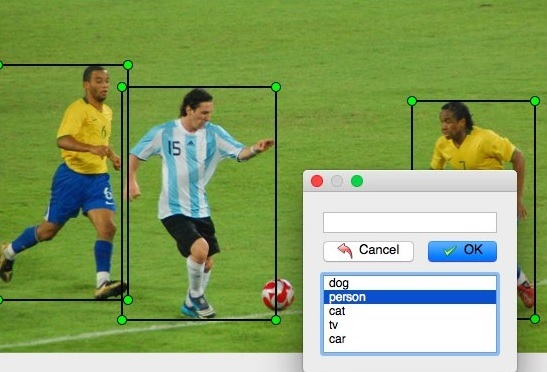
\includegraphics[scale=0.7]{Sources/labelimg.jpg}
	\caption{Vorbereitung der Datensätzen mit dem Labelimg Programm \cite{labelimg2019}}
	\label{img:labelimg}
\end{figure}
Eine Klassifizierung gehört zum überwachten Lernen und benötigt deswegen gelabelte Datensätze. Das Labeln wurde mit dem Open Source Programm \textit{LabelIMG} \cite{labelimg2019} durchgeführt. Dabei wird das zu trainierende Objekt mit einem rechteckigen Kasten umschlossen und einer Klasse auf den Bildern markiert. Diese Daten werden zunächst in einer XML Datei abgespeichert. 
  \subsection{Mean average Precision}\label{s.map}
Oft können neuronale Netze nicht nur ein Objekt gleichzeitig erkennen, sondern geben als Ergebnis mehrere Hypothesen aus. Dadurch entsteht das Problem, dass nicht mehr nur zwischen richtig und falsch unterschieden werden kann, sondern eine Genauigkeit benötigt wird, welche alle möglichen Objekte einbezieht. Eine Metrik, welche auf diese Informationen eingeht, ist die (mean) average Precision (AP/mAP). Für die Berechnung wird die Präzision (Precision) und der Rückgabewert eines Ergebnisses benötigt. Die Präzision $P$ beschreibt den Anteil der richtig erkannten Objekte unter allen erkannten Objekten. Der Rückgabewert $R$ (Recall) ist der korrekte Anteil von allen möglichen Objekten. Formell ausgedrückt:
\begin{eqnarray}
P&=&\frac{richtig\medspace erkannte}{richtig\medspace erkannte + falsch\medspace erkannte}\\
R&=&\frac{richtig\medspace erkannte}{richtig\medspace erkannte + falsche\medspace nicht\medspace erkannte}
\end{eqnarray}
Häufig wird ein Schwellwert für die Pseudowahrscheinlichkeit genutzt, mit welchem entschieden wird, wann ein erkanntes Objekt der Rückgabeliste hinzugefügt wird oder nicht. Wird der Schwellwert niedrig angesetzt, werden meist mehr Objekte, als \textit{erkannt} eingestuft. Dadurch steigt der Rückgabewert mit richtig erkannten Objekten. Gleichzeitig sinkt aber auch die Präzision da natürlicherweise auch mehr falsche Objekte erkannt werden. Objekterkennungsverfahren mit einer hohen Qualität zeigen aber weiterhin eine gute Präzision.
\section{Arten der Farbnormalisierung}\label{s.farbnormalisierungen}  
Die Farbnormalisierung ist ein Thema der Bildverarbeitung welches sich hauptsächlich mit künstlicher Farbsicht befasst. Die Verteilung und Darstellung von Farben auf Bildern hängt hauptsächlich von Beleuchtungsbedingungen und der Kamera ab. Das bedeutet, dass sich die Farben bei der Aufnahme, je nach Beleuchtung, verändern. Das ist gerade im Bereich von \textit{Maschine Learning} problematisch, da diese Farbveränderungen zu Fehlern im Lernprozess und der späteren Genauigkeit führen. Farbnormalisierung-Algorithmen, sollen dafür sorgen, dass die Farbabweichungen durch Lichteinfluss geringere Auswirkungen haben und zu besseren Ergebnissen führen. Im Folgenden werden die ausgewählten Algorithmen erläutert, welche im Rahmen dieser Arbeit getestet werden.
  \subsection{Ansatz des Gray-World-Algorithmus}\label{s.gw}
Bei der Gray-World-Normalisierung \cite{buenaposada2001variations} geht es nicht, wie der Name vermuten lässt, um die Umwandlung in ein Graustufenbild, eher werden die verschieden Farbräume abgedunkelt und eingegrenzt. Wenn über die Farben in einem Bild keine Annahmen getroffen werden können, wird davon ausgegangen, dass sich die Farbwerte in einem Bild sich vektoriell zu Grau addieren, also das der Mittelwert vom Bild Grau ist. Sollte das nicht der Fall sein, wird davon ausgegangen, dass das auf eine Farbige Beleuchtung zurückzuführen ist und normalisiert das Bild so, dass die Graue-Welt-Theorie erfüllt wird. Die Farbkanäle werden durch einen Skalierungsfaktor normalisiert, so das der Mittelwert 128 entspricht. Es werden somit Farbstiche herausgefiltert. Wie schon erwähnt, ist diese Art der Farbnormalisierung für verschiedene Farbvariationen unveränderlich. Ein Problem dieses Normalisierungsverfahrens besteht darin, dass es nicht einfach für dynamische Szenen verwendet werden kann. Um solche Probleme zu lösen, gibt es mehrere Ansätze dieser Ausgleichung.
\begin{align} \label{f:gw} (\alpha R, \beta G, \gamma B) \rightarrow\left(\frac{\alpha R} {\frac{\alpha}{n} \sum_{i} R}, \frac{\beta G} {\frac{\beta}{n} \sum_{i} G}, \frac{\gamma B} {\frac{\gamma}{n} \sum_{i} B} \right) \end{align}
Eine Veränderung der Beleuchtungsfarbe kann als Skalierung von $\alpha$, $\beta$ und $\gamma$ für die R-, G-, und B-Kanäle modelliert werden (\ref{f:gw}). Als solcher ist der Gray-World für die Variationen der Beleuchtungsfarbe unveränderlich. Dieses Vorgehen berücksichtigt aber nicht alle Intensitäten der Beleuchtungsintensität und ist nicht für Dynamische Szenen geeignet. Aus diesem Grund, gibt es verschiedenste Ansätze dieses Verfahrens.
  \subsection{Ansatz der Histogramm-Ausgleichung}\label{s.ha}  
Die Histogramm-Ausgleichung \cite{goatman2003colour} ist eine nichtlineare Transformation, welche auf Grundlage der Histogramme arbeitet. Der Pixelrang wird dabei nicht verändert und kann bei jeder monoton steigenden Farbformation verwendet werden. Dieses Normalisierungsverfahren wird besser als der Gray-World-Algorithmus angesehen, da nicht nur die Farbkanäle beeinflusst werden, sondern die Farbverteilung in den Bildern. Durch die Histogramm-Ausgleichung entsteht ein dominanter blauer Kanal, wodurch das Bild oft unnatürlich erscheint.
   \begin{table}
  [h]
  \centering
  \caption{Pixelbild in ein tabellarisches Histogramm überführt}
  \label{tab:bildha}
  \begin{minipage}{\textwidth}
  \center
  \begin{tabular}{|c|c|c|c|c|c|c|c|}
  \hline
  0&1&5&1&7&2&0&3\\
  \hline
  0&0&5&5&5&2&4&5\\
  \hline
  4&5&1&4&1&5&1&4\\
  \hline
  5&1&2&4&5&2&6&3\\
  \hline
  5&2&6&4&0&4&0&5\\
  \hline
  4&0&2&4&7&4&6&2\\
  \hline
  5&1&6&1&0&1&1&5\\
  \hline
  4&5&2&4&2&5&2&5\\
  \hline
  \end{tabular}
  \end{minipage}
  \begin{minipage}{\textwidth}
  \hspace{\textwidth}
  \end{minipage}
  \begin{minipage}{\textwidth}
  \center
  \begin{tabular}{|l|c|c|c|c|c|c|c|c|}
  \hline
  Graustufen & 0 & 1 & 2 & 3 & 4 & 5 & 6 & 7\\
  \hline
  Anzahl der Pixel & 8 & 10 & 10 & 2 & 12 & 16 & 4 & 2\\
  \hline
  \end{tabular}
  \end{minipage}
  \end{table}
Für die Mathematische Herleitung, betrachten wir zunächst ein Graustufenbild $X$ und geben mit $n_{i}$ die Anzahl der Graustufen an, wobei $i$ die Häufigkeit des auftretenden Pixels ist. Zu sehen in der Funktion \ref{f:ha1}.
\begin{eqnarray} \label{f:ha1} p_{x}(i)=p(x=i)&=&\frac{n_{i}}{n}, 0\leq i \leq L \end{eqnarray}
$L$ ist die Gesamtzahl aller Graustufen im Bild (normalerweise 256), $n$ ist die Gesamtzahl der Pixel im Bild und $p_{x}(i)$ welches das normalisierte Histogramm für den Pixelwert $i$ ist. Die Definition der Verteilungsfunktion kann man in \ref{f:ha2} sehen:
\begin{eqnarray} cdf_{x}(i) &=& \sum_{j=0}^i p_{x}(j)\end{eqnarray}
Um die Funktionsweise etwas verständlicher zu machen, folgt ein kleines Beispiel. Dafür haben wir ein 8x8 Bild (Tabelle \ref{tab:bildha}), mit 8 Graustufen. Die Pixelverteilung wird in dem Tabellarischen Histogramm zusammengefasst.  
Aus der Pixelverteilung wird nun ein Ausgleich berechnet welche den kumulativen Pixelwert durch die Anzahl aller Pixel teilt und das Ergebnis wiederum durch die höchste Graustufe. Das wird für jede wird für jede Grauabstufung durchgeführt, wie in Tabelle \ref{tab:haberechnung} beschrieben.
 Das Ergebnis wird nun gerundet und der passenden Graustufe zugeordnet. Die Vorgehensweise mit Farbbildern funktioniert gleich, nur dass die R, G und B Kanäle verwendet werden. Häufig wird für diese Verfahren, ein Farbraum gewählt, welcher einen Kanal für die Luminanz besitzen.
  \begin{table}
  [h]
  \caption{Mathematische Umsetzung der Histogrammausgleichung}
  \label{tab:haberechnung}
  \centering
  \begin{tabular}{|l|c|c|c|c|}
  \hline
  $r_{k}$ & $P_{k}$ & Kumulative Werte & $Kumulative/Gesamt*(L-1)$ & Gerundete nahe Grauwerte\\
  \hline
  0 & 8 & 8 & $8/64*7=0.875$ & 1\\
  \hline
  1 & 10 & 18 & $18/64*7=1.968$ & 2\\
  \hline
  2 & 10 & 28 & $28/64*7=3.0625$ & 3\\
  \hline
  3 & 2 & 30 & $30/64*7=3.2812$ & 3\\
  \hline
  4 & 12 & 42 & $42/64*7=4.5937$ & 5\\
  \hline
  5 & 16 & 58 & $58/64*7=6.3437$ & 6\\
  \hline
  6 & 4 & 62 & $62/64*7=6.78125$ & 7\\
  \hline
  7 & 2 & 64 & $64/64*7=7$ & 7\\
  \hline
  \end{tabular}
  \end{table}
Die Graustufen werden im weiteren Schritt übernommen und in Das Quellbild eingesetzt. Dabei verschieben sich die Grauwerte so, das den Gerundeten Grauwerten aus Tabelle \ref{tab:haberechnung} entsprechen. Das Ausgeglichen Bild kann man in der Tabelle \ref{tab:hamatrix} betrachten. 
\begin{table}[htb]
  \caption{Bildmatrix des Ausgeglichenen Histogramms}
  \label{tab:b1}
  \centering
  \begin{minipage}{\textwidth}
  \center
  \begin{tabular}{|c|c|c|c|c|c|c|c|}
  \hline
  1&2&6&2&7&3&1&3\\
  \hline
  1&1&6&6&6&3&5&6\\
  \hline
  5&6&2&5&2&6&2&5\\
  \hline
  6&2&3&5&6&3&7&3\\
  \hline
  6&3&7&5&1&5&1&6\\
  \hline
  5&1&3&5&7&5&7&3\\
  \hline
  6&2&7&2&1&2&2&6\\
  \hline
  5&6&3&5&3&6&3&6\\
  \hline
  \end{tabular}
  \end{minipage}
  \begin{minipage}{\textwidth}
  \hspace{\textwidth}
  \end{minipage}
  \begin{minipage}{\textwidth}
  \center
  \begin{tabular}{|l|c|c|c|c|c|c|c|c|}
  \hline
  Graustufen & 0 & 1 & 2 & 3 & 4 & 5 & 6 & 7\\
  \hline
  Anzahl der Pixel & 0 & 8 & 10 & 12 & 0 & 12 & 16 & 6\\
  \hline
  \end{tabular}
  \end{minipage}
  \end{table}
  \newpage
  \subsection{Ansatz der Histogramm-Spezifikation}\label{s.hs}
Ähnlich wie die Histogramm-Ausgleichung arbeitet die Histogramm-Spezifikation\\ \cite{goatman2003colour}. Die Histogramme der roten, grünen und blauen Kanäle werden so umgewandelt, dass sie den Formen von drei spezifischen Histogrammen entsprechen, anstatt sie einfach auszugleichen. Mithilfe dieses Vorgehens wird darauf abgezielt, Bilder zu erhalten, welche ein Histogramm einer bestimmten Farbverteilung hat. Zunächst muss das Bild so konvertiert werden, dass das Histogramm eine bestimmte Farbverteilung hat. Für diese Methode werden üblicher weise zwei ähnliche Bilder verwendet, einmal das Quellbild und das Referenzbild. Das Referenzbild hat die gewünschte Form des Histogramms, hingegen das Quellbild angepasst werden soll. Häufig wird zunächst eine Histogramm-Ausgleichung der beiden Bilder durchgeführt. Es kann aber auch mit den Originalbilder durchgeführt werden. Im Weiteren wird das Histogramm des Quellbildes auf das Histogramm des Referenzbildes angepasst. Die mathematische Herleitung beginnt auch hier mit einem Grasstufeneingabebild $S$. 
Diese Bild hat eine Wahrscheinlichkeitsdichtefunktion $p_{r}(r)$, wobei $r$ ein Graustufenwert ist und $p_{r}(r)$ die Wahrscheinlichkeit für diesen Wert darstellt. Diese Wahrscheinlichkeit kann aus dem Histogramm des Bildes Berechnet werden:
\begin{eqnarray} p_{r}(r_{j})&=&\frac{n_{j}}{n} \end{eqnarray}
Dabei ist $n_{j}$ die frequenz des Graustufenwerts $r_{j}$ und $n$ die Gesamtzahl der Pixel im Bild. Bei betrachtung der gewünschten Ausgabewahrscheinlichkeitsdichtefunktion $p_{z}(z)$. Eine Transformation von $p_{r}(r)$ wird durchgeführt, damit es nach $p_{z}(z)$ anzupassen. Gegeben sind die Funktionen der beiden Bilder: 
\begin{align} \label{f:quell} S(r_{k})=\sum_{j=0}^k p_{r}(r_{j}) ,& &k=0,1,2,3,4,..,L\end{align}
\begin{align} \label{f:referenz} G(z_{k})=\sum_{j=0}^k p_{z}(z_{j}) ,& &k=0,1,2,3,4,.., L \end{align}
Dabei stellt $S$ das Quellbild (\ref{f:quell}) und $G$ das Referenzbild (\ref{f:referenz}) dar. $k$ beinhaltet alle Graustufen bis hin zur höchsten $L$.   
Auch in dieser Herleitung bildet die Gesamtzahl an Graustufen (Normalerweise 256). Im weiteren wird versucht, jeden $r$-Wert in $S$ auf den $z$-Wert von $G$ abzubilden, welche die gleiche Wahrscheinlichkeit haben. Das heißt:
\begin{align} S(r_{j})=G(z_{i})& &oder& & z=G^{-1}(S(r)) \end{align} 
Um die Funktionsweise verständlicher darzustellen, wird kurz auf das Vorgehen und die mathematische Herleitung eingegangen. Dafür gibt es in den Tabellen \ref{tab:b1} und \ref{tab:b2} zwei Histogramme mit 8 Grauabstufungen. In diesen Tabellen wird aufgeführt, wie oft der jeweilige Grauwert in dem Bild vorkommt. 
  \begin{table}[htb]
  \caption{Tabellarisches Histogramm des Quell-Bildes (B1)}
  \label{tab:b1}
  \centering
  \begin{minipage}{\textwidth}
  \center
  \begin{tabular}{|c|c|c|c|c|c|c|c|}
  \hline
  0&1&5&1&7&2&0&3\\
  \hline
  0&0&5&5&5&2&4&5\\
  \hline
  4&5&1&4&1&5&1&4\\
  \hline
  5&1&2&4&5&2&6&3\\
  \hline
  5&2&6&4&0&4&0&5\\
  \hline
  4&0&2&4&7&4&6&2\\
  \hline
  5&1&6&1&0&1&1&5\\
  \hline
  4&5&2&4&2&5&2&5\\
  \hline
  \end{tabular}
  \end{minipage}
  \begin{minipage}{\textwidth}
  \hspace{\textwidth}
  \end{minipage}
  \begin{minipage}{\textwidth}
  \center
  \begin{tabular}{|l|c|c|c|c|c|c|c|c|}
  \hline
  Graustufen & 0 & 1 & 2 & 3 & 4 & 5 & 6 & 7\\
  \hline
  Anzahl der Pixel & 8 & 10 & 10 & 2 & 12 & 16 & 4 & 2\\
  \hline
  \end{tabular}
  \end{minipage}
  \vspace{-1 cm}
  \end{table}
  \begin{table}
  [h]
  \caption{Tabellarisches Histogramm des Referenz-Bildes (B2)}
  \label{tab:b2}
  \centering
  \begin{minipage}{\textwidth}
  \center
  \begin{tabular}{|c|c|c|c|c|c|c|c|}
  \hline
  4&6&5&6&6&7&5&5\\
  \hline
  5&5&4&4&4&7&4&4\\
  \hline
  5&6&4&5&5&6&6&5\\
  \hline
  5&4&7&4&5&4&6&7\\
  \hline
  4&5&5&5&4&4&6&5\\
  \hline
  6&5&4&5&6&6&7&4\\
  \hline
  6&4&5&4&7&4&6&5\\
  \hline
  7&6&6&5&4&5&6&7\\  
  \hline
  \end{tabular}
  \end{minipage}
  \begin{minipage}{\textwidth}
  \hspace{\textwidth}
  \end{minipage}
  \begin{minipage}{\textwidth}
  \center
  \begin{tabular}{|l|c|c|c|c|c|c|c|c|}
  \hline
  Graustufen & 0 & 1 & 2 & 3 & 4 & 5 & 6 & 7\\
  \hline
  Anzahl der Pixel & 0 & 0 & 0 & 0 & 20 & 20 & 16 & 8\\
  \hline
  \end{tabular}
  \end{minipage}
  \end{table}\\
Nun werden die Histogramme, wie in Abschnitt \ref{s.ha} beschrieben, ausgeglichen. Von 0 bis $L-1$ werden die Summen der Pixel berechnet, durch die Anzahl der im Bild enthaltenden Pixel geteilt und mit der höchsten Graustufe $(L-1)$ multipliziert. Das Ergebnis des Ausgleiches ist in Tabelle \ref{tab:hs} dargestellt.
\begin{table}
  [h]
  \caption{Von zwei ausgeglichenen Histogrammen zu einem spezifizierten Histogramm}
  \label{tab:hs}
  \centering
  \begin{tabular}{|c|c|c|c|}
  \hline
  Graustufe & Ausgleichung B1 & Ausgleichung B2 & Spezifiziertes Histogramm\\
  \hline
  0 & 1 & 0 & 4\\
  \hline
  1 & 2 & 0 & 4\\
  \hline
  2 & 3 & 0 & 5\\
  \hline
  3 & 3 & 0 & 5\\
  \hline
  4 & 5 & 2 & 6\\
  \hline
  5 & 6 & 4 & 6\\
  \hline
  6 & 7 & 6 & 7\\
  \hline
  7 & 7 & 7 & 7\\
  \hline
  \end{tabular}
  \end{table}
Nun werden die Grauwertverteilungen von B1 und die Verteilung von B2 angepasst. Dafür wird der nächste Wert aufgerundet von B1 übernommen.\\\\
In einem Beispiel von Tabelle \ref{tab:hs}: \\
Bei Graustufe 0 liegt der Wert von B1 bei 1. Der nächst höhere Wert in B2 liegt bei 2 an der Graustufe 4. Dieser Wert wird in das Zielhistogramm übernommen. Dabei werden alle Pixel welche vorher den Grauwert 0 haben in den Grauwert 4 Übertragen. Diese Prinzip, wird für jeden Farbwert des Histogramms durchgeführt.\\\\
Aus der neuen Stufen-Verteilung entsteht ein neues Histogramm (Tabelle \ref{tab:B3}), welches Ähnlichkeiten zum Referenz-Histogramm hat. Dadurch verschiebt sich das Histogramm Richtung Weiß und das Bild wird erhellt.
  \begin{table}
  [h]
  \caption{Tabellarisches Histogramm des Quell-Bildes (B1) auf Basis des Referenz-Bildes (B2)}
  \label{tab:B3}
  \centering
  \begin{minipage}{\textwidth}
  \center
  \begin{tabular}{|c|c|c|c|c|c|c|c|}
  \hline
  4&4&6&4&7&5&4&5\\
  \hline
  4&4&6&6&6&5&6&6\\
  \hline
  6&6&4&6&4&6&4&6\\
  \hline
  6&4&5&6&6&5&7&5\\
  \hline
  6&7&7&6&4&6&4&6\\
  \hline
  6&4&7&6&7&6&7&7\\
  \hline
  6&4&7&4&4&4&4&6\\
  \hline
  6&6&5&6&5&6&5&6\\
  \hline
  \end{tabular}
  \end{minipage}
  \begin{minipage}{\textwidth}
  \hspace{\textwidth}
  \end{minipage}
  \begin{minipage}{\textwidth}
  \center
  \begin{tabular}{|l|c|c|c|c|c|c|c|c|}
  \hline
  Graustufen & 0 & 1 & 2 & 3 & 4 & 5 & 6 & 7\\
  \hline
  Anzahl der Pixel & 0 & 0 & 0 & 0 & 18 & 12 & 28 & 6\\
  \hline
  \end{tabular}
  \end{minipage}
  \end{table}
	
	% Die Zähler für Tabellen und Abbildungen werden zurückgesetzt, damit
	% in jedem Kapitel die Nummerierung neu beginnt
\setcounter{table}{1}
\setcounter{figure}{1}
	% Einbinden des dritten Kapitels
	%!TEX root = ../draft.tex
\chapter{Methodik und Durchführung}\label{s.methudurchf}
In diesem Kapitel werden die verwendeten Datensätze aufgeführt und die Umsetzung der Normalisierungsalgorithmen beschrieben.  
 \section{Vortrainierte Netze}\label{s.modell}
Das Unternehmen COCO \cite{common2018data} (Common Objects in Contexts) stellt eine Vielzahl an Datensätzen bereit mit denen neuronale Netze trainiert werden können. Bei den Datensäzen handelt es sich um unterschiedliche Objekte in verschiedenen Umgebungen.  
Einige Netze welchem mit dem COCO datensätzen traniert wurden stehen als \textit{Open Source} zur Verfügung. Die folgende Tabelle \ref{tab:cocomodels} führt ausgewählte neuronale Netze auf, um die Genauigkeit und Geschwindigkeit vergleichen zu können, damit ein geeignetes Netz für die Versuche ausgewählt werden kann.
\begin{table}
[h]
\caption{Künstliche neuronale Netze \cite{google2018tens} welche mit dem COCO Dataset Trainiert wurden \cite{common2018data}} 
\label{tab:cocomodels}
\centering
\begin{tabular}{|l|c|c|}
\hline
Neuronales Netz & mAP & Geschwindigkeit\\
\hline
faster\_rcnn\_inception\_v2\_coco & 28 & 58\\
faster\_rcnn\_resnet50\_coco & 30 & 89\\
rfcn\_resnet101\_coco & 30 & 92\\
ssd\_mobilenet\_v1\_coco & 30 & 21\\
ssd\_resnet\_50\_fpn\_coco & 35 & 76\\
\hline
\end{tabular}
\end{table}
Um die Auswirkungen der Normalisierung deutlich hervorheben zu können wurde bei der Auswahl des Netzes eins ausgewählt, welches eine recht niedrige mAP hat. Weshalb das faster\_rcnn\_inception\_v2\_coco ausgewählt wurde. Dieses hat eine \textit{mAP} von 28 und eine Geschwindigkeit von 32 ms. Dadurch das es die niedrigste \textit{mAP} hat, sollten die Auswirkungen, der Normalisierungsverfahren, in der Genauigkeit stärker ersichtlich werden. Das ausgewählte Netz wird im folgenden auf die Datensätze, welche im anschließenden Unterkapitel aufgeführt sind.
  \section{Trainingsdaten}\label{s.tdaten}
Wie bereits in Kapitel \ref{s.trainingsdaten} beschrieben werden zum trainiren eines Neuronalen üblicherweise mehere Hunderttaused Daten benötigt. Durch die Verwendung eines vortrainierten Netzes, werden für das trainieren der eigenen Klassen nur noch durchschnittlich 150 Bilder pro Objektklasse benötigt was die Trainingsdauer deutlich verkürzt. Die Bilder der eigenen Daten werden mit einer 13 Megapixel Kamera eines \textit{Huawei P Smart} aufgenommen. Die verwendeten Objekte werden von vielen verschiedenen Seiten aufgenommen. Da die Bilder erstellten Bilder mehrere Megabyte groß waren, müssten diese auf 100-300 KB komprimiert werden.\\ %Warum müssen die das? 
Damit am Ende des Projektes möglichst gute Vergleichswerte entstehen, werden mehrere Datensätze vor den Versuch verwendet. Insgesamt werden die neuronalen Netze mit 3 unterschiedlichen Datensätzen trainiert. Dafür wurden 3 Datensätze heraus gesucht. Der erste Datensatz welcher getestet wird, ist der Nahrungsmittel Datensatz eines früheren Projektes, zum anderen der Datensatz von \textit{Pascal Visual Object Classes} (PascalVOC) und der Hunderassen Datensatz, Stanford Dog Dataset.\\
In den folgenden Tabellen werden alle Datensätze mit den zugehörigen Klassen und Anzahl an Trainingsbildern aufgeführt:\\\\
Der erste Datensatz besteht aus 6 Klassen welche in der Tabelle \ref{tab:nahrungsmittel} aufgeführt sind. Jede klasse besitzt um die 100-150 Bilder welche zusätzlich Annotations-Dateien mit den Koordinaten der Klassifizierungsboxen (Kapitel \ref{s.trainingsdaten}) beinhalten. Dieser Datensatz ist mit seinen ca. 1000 Bildern der kleinste Datensatz. 
\begin{table}
[h]
\caption{Datensatz mit Nahrungsmitteln}
\centering
\begin{tabular}{|l|l|}
\hline
Klassenname & Klassenname\\
\hline
Milch - Packung & Orangensaft - Packung\\
Wasser - Flasche & Bier - Flasche\\
Brunch - Aufstrich & Margarine - Aufstrich\\
\hline
\end{tabular}
\label{tab:nahrungsmittel}
\end{table}
Der PascalVOC Datensatz umfasst 20 Klassen und besteht aus 5.000 Bildern. Von 2005 bis 2012 wurde jährlich die PascalVOC Challenges durchgeführt. Dabei sollte das beste verfahren für die Segmentierung, Klassifikation und Objekterkennung ermittelt werden. Inhaltlich befasst sich der Datensatz mit einer reihe unterschiedlicher Klassen, welche in Tabelle \ref{tab:pvoc} zu erkennen sind. Es gibt einige Unterschiede in der Häufigkeit der auftretenden Klassen. Beispielsweise sind in rund 2000 Bildern insgesamt 4.690 Personen enthalten, weswegen es möglicherweise Unterschiede in der Genauigkeit untereinander, der Klassen geben könnte. Die Aufnahmen der Bilder sind thematisch und und von der Art der Aufnahme unstrukturiert, was bedeutet, dass teilweise Bilder von einzelnen Objekten, Gruppen von Objekten oder auch ganze Szenen enthalten sind.
\begin{table}
[h]
\caption{Pascal Visual Object Classes \cite{pascal-voc-2007}}
\centering
\begin{tabular}{|l|l|l|l|}
\hline
Klassenname & Klassenname & Klassenname & Klassenname\\
\hline
Person & Vogel & Katze & Kuh\\
Hund & Pferd & Schaf & Zug\\
Flugzeug & Fahrrad & Boot & Bus\\
Auto & Motorrad & Flasche & Stuhl\\
Tisch & Blumentopf & Sofa & Bildschirm\\
\hline
\end{tabular}
\label{tab:pvoc}
\end{table}
Der dritte Datensatz welcher in dieser Arbeit verwendet wird, ist der Hunde Datensatz aus Stanford und beinhaltet 120 verschiedene Hunderassen. Jede Klasse hat um die 200 Bilddaten. Wegen der Struktur des Datensatzes, in einzelnen Ordnern, kann eine Auswahl der priorisierten Hunderassen zusammengestellt werden. Für den Versuch und damit eine bessere Übersicht erreicht werden kann, wurden 20 Hunderassen ausgewählt. Die Anotationen der Daten sind in Form von XML Dateien beigefügt. In der Tabelle \ref{tab:sdd} werden die ausgewählten Klassen des Datensatzes zusammengefasst.
\begin{table}
[h]
\caption{Stanford Dog Dataset \cite{KhoslaYaoJayadevaprakashFeiFei_FGVC2011}}
\label{tab:sdd}
\centering
\begin{tabular}{|l|l|l|l|}
\hline
Klassenname & Klassenname & Klassenname & Klassenname\\
\hline
Chihuahua & Japanese Spaniel & Maltese Dog & Pekinese\\
Shih-Tzu & Blenheim Spaniel & Papillon & Toy Terrier\\
Rhodesian Ridgeback & Afghan Hound & Basset & Beagle\\
Bloodhound & Bluetick & Coonhound & Walker Hound\\
Redbone & Borzoi & Irish Wolfhound & Italian Greyhound\\
\hline
\end{tabular}
\end{table}
Von der Struktur der Datensätze, sind sie ähnlich aufgebaut. Viele verschiedene Klassen mit verschiedenen Szenen und Kontexten. Im weiteren wird zunächst auf die Umsetzung der Normalisierungsverfahren eingegangen, um weiter Erkenntnisse zu erlangen.
\section{Normalisierung-Algorithmen}\label{s.nalgorithmen}
Für die Normalisierung der Datensätze ist eine Methode nötig, um mehrere Bilder möglichst schnell hintereinander zu bearbeiten. Für die Normalisierung wurden Python Programme geschrieben, welche nacheinander die Bilder, anhand eines Algorithmus verarbeitet. Dafür wurde mit unter die \textit{Python Image Libary} und OpenCV genutzt. Beide Bibliotheken werden für das verarbeiten von Bildern benötigt. 
%Seitenumbruch
\subsection{Gray-World-Algorithmus} %Bessere variablen namen wären schön um die lesbarkeit zu erhöhen z.b img statt ning, avarage_green_channel ...  V
\begin{lstlisting}
# Importieren des Bildes
nimg = cv.imread(i, 1)
# Umwandlung des Bildes und der Kanäle in 32 Bit
nimg = nimg.transpose(2, 0, 1).astype(np.uint32)
# Zwischenspeichern des durchschnittlichen Grünkanals
mu_g = np.average(nimg[1])
# Berechnng des rot-Kanals: 
nimg[0] = np.minimum(nimg[0]*(mu_g/np.average(nimg[0])),255)
# Berechnung des blau-Kanals:
nimg[2] = np.minimum(nimg[2]*(mu_g/np.average(nimg[2])),255)
Umwandlung des Bildes in 8 Bit
img_output = nimg.transpose(1, 2, 0).astype(np.uint8)
\end{lstlisting}
Der Gray World Algorithmus \cite{gray2012world} welcher verwendet wird, funktioniert etwas anders als in den Grundlagen beschrieben. Für die Normalisierung der Kanäle, wird der durchschnitt des Grünkanal verwendet, da diese Farbe wichtig für das Helligkeitsempfinden ist. % Was ist der unterschied wird hier nicht nur ein anderer Farbkanal als Grau genommen? Verweise auf den Quellcode wären schon "In Zeile 1 wird
In der Zeile 2 wird der Farbraun des Bildes in 32 Bit umgewandelt. Daraufhin wird in Zeile 6 der Durchschnittswert des Grünkanals berechnet und zwischengespeichert. In der Zeile 8 wird der Grün-Kanal nun mit dem durchschnitt des Rot-Kanals dividiert und anschließend mit dem Minimum des Rot-Kanals multipliziert und übernommen. Der gleiche Vorgang folgt mit dem Blau-Kanal in Zeile 10. Abschließend wird das bearbeitete Bild in 8 Bit gewandelt und ausgegeben (Abbildung \ref{img:gwnimg}). Für das verfahren wird keine spezielle Python Bibliothek eingesetzt. %Weißt du warum das bild erst auf 32 bit hoch skalliert wird und dann auf 8 bit zurück, hatte auch nicht gedacht das das Bild am anfand nur 8 Bit hatte ...
\begin{figure}
	[h]
	\centering
	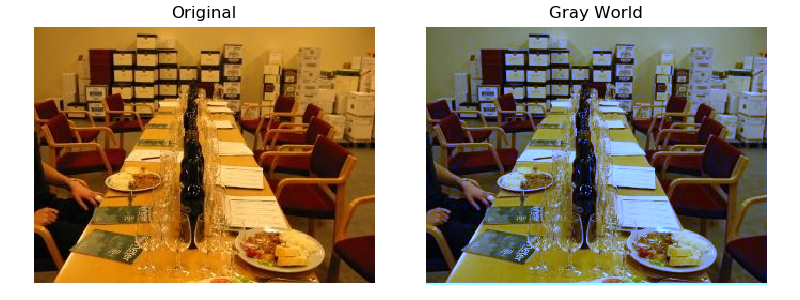
\includegraphics[scale=0.6]{Sources/gwn.png}
	\caption{Auswirkung des Gray-World Algorithmus}
	\label{img:gwnimg}
\end{figure}
%Seitenumbruch da ansonten der Alogorythmus auf zwei seiten steht
\subsubsection{Histogramm Ausgleich}
\begin{lstlisting}
# Importieren des Bildes
img = cv.imread('input.jpg')
img_yuv = cv.cvtColor(img, cv.COLOR_BGR2YUV)
img_yuv[:,:,0] = cv.equalizeHist(img_yuv[:,:,0])
img_output = cv.cvtColor(img_yuv, cv.COLOR_YUV2BGR)
\end{lstlisting}
Für die Histogramm Ausgleichung \cite{histogram2012equalisation} wird das Bild in Zeile 3 vom BGR Farbraum in den YUV Farbraum (Kapitel \ref{s.lab} umgewandelt. Der Y-Kanal wird für die Histogramm Ausgleichung verwendet. Das hat den Grund, dass das Luminanzsignal oder auch Leuchtdichte-Signal die Summe der drei Grundfarben Rot Grün und Blau und die Helligkeitsinformation enthält. In Zeile 4 wird das Histogramm des Y Kanals, wie in Kapitel \ref{s.histogramme} beschrieben, ausgeglichen. Das normalisierte Bild wird von dem YUV Farbraum zurück in den BGR Farbraum konvertiert und zwischengespeichert. Das Ergebnis wird als Bild ausgegeben (Abbildung \ref{img:histogrameq}).
\begin{figure}
	[h]
	\centering
	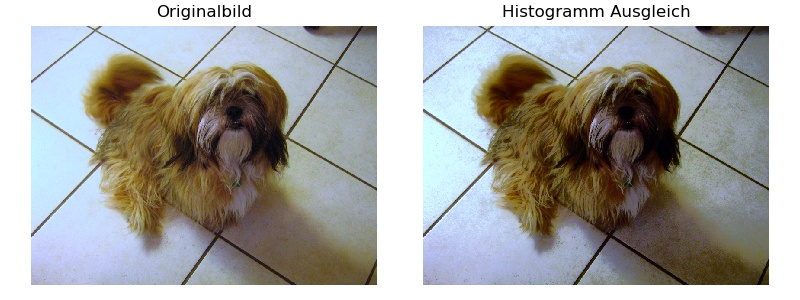
\includegraphics[scale=0.7]{Sources/histeq.jpg}
	\caption{Auswirkung der Histogramm Ausgleichung}
	\label{img:histogrameq}
\end{figure}	
\subsection{Histogramm Spezifikation}
\begin{lstlisting}
# Importieren des Referenzbildes
reference = io.imread('reference.jpg')
image = io.imread('image.jpg')
matched = match_histograms(image, reference, multichannel=True)
\end{lstlisting}
Der dritte Normalisierungsfunktion welche für die Datensätze angewendet wird, ist die Histogramm Spezifikation (Kapitel \ref{s.hs}) oder auch \textit{Histogramm Matching}. Für den Algorithmus wird die Python Bibliothek \textit{Scikit-image} verwendet. Dafür werden ein Referenzbild und ein Zielbild geladen. Diese beiden Bilder, werden mit der Funktion \textit{match\_histograms} verarbeitet. Das Zielbild wurde auf das Histogramm des Referenzbildes angepasst. In dem Beispiel \ref{img:histogramspez} kann man gut erkennen, das das Quellbild, welches stark verdunkelt ist, durch ein gut ausgeleuchtetes Referenzbild, eine wesentlich bessere Helligkeit aufweist (Abbildung \ref{img:histogramspez}). Die Problematik bei dieser Normalisierungs Methode besteht darin, das ein einheitliches Referenzbild genutzt werden muss auf welchem dann der gesamte Datensatz Normalisiert wird.
\begin{figure}
	[h]
	\centering
	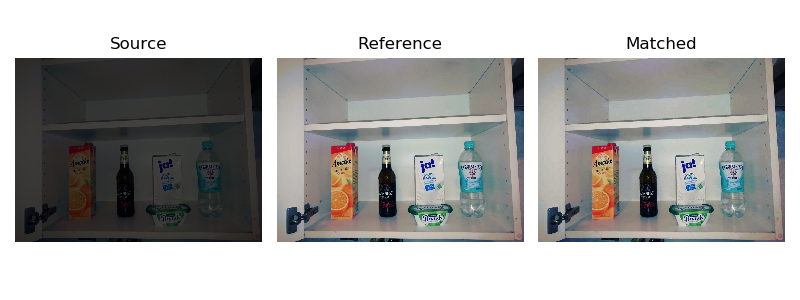
\includegraphics[scale=0.6]{Sources/HS_beispiel.png}
	\caption{Das Zielbild wurde mithilfe des Referenzbildes ausgeglichen und angepasst. Auf der linken Seite ist das Ergebnis der Spezifikation}
	\label{img:histogramspez}
\end{figure}
	
	% Die Zähler für Tabellen und Abbildungen werden zurückgesetzt, damit
	% in jedem Kapitel die Nummerierung neu beginnt
\setcounter{table}{1}
\setcounter{figure}{1}
	% Einbinden des dritten Kapitels
	%!TEX root = ../draft.tex
\chapter{Ergebnisse}\label{s.ergebnisse}
Nachdem alle Trainingseinheiten mit den verschiedenen Normalisierungsverfahren durchlaufen wurden, sollen die Ergebnisse aufgeführt und verglichen werden. Zunächst wird auf die Entwicklungsumgebung beschrieben und im Anschluss auf die Ergebnisse der Auswertung. Als Vergleichswerte konnte mithilfe von Tensorboard die Genauigkeiten des Netzes erhoben werden. Jede Klasse hat eine eigene durchschnittliche Genauigkeit (AP) und eine Genauigkeit für das gesamte Netz in Form einer mAP. In den folgenden Tabellen werden bestimmte Abkürzungen verwendet: N = Normaler Datensatz, GW = Gray-World-Algorithmus, HA = Histogramm Ausgleich, HS = Histogramm Spezifikation (Die besten Ergebnisse einer Klasse wurden durch Fettschrift hervorgehoben) 
\section{Frameworks und Entwicklungsumgebung}\label{s.entwicklung}
Wie in vorherigen Kapiteln schon beschrieben ist das Trainieren eines künstlichen neuronalen Netzes oder eines faltenden neuronalen Netzes sehr rechenintensiv. Die enthaltenen Daten werden parallel mittels Matrizenmultiplikation verarbeitet. Aus diesem Grund werden für die Verarbeitung Grafikprozessoren hauptsächlich verwendet da diese im Gegensatz zu normalen Prozessoren für die Berechnung von Matrizen konzipiert wurden.\\
Auf Softwareseite gibt es eine Menge an Frameworks, mit welcher sich CNNs realisieren lassen. Einige von denen sind beispielsweise Tensorflow, Keras und Theano. Wegen der vorliegenden Erfahrung und der Möglichkeit Trainingsfortschritte grafisch anzeigen zu können, wird der praktische Teil der Arbeit mittels Tensorflow durchgeführt. Tensorflow ist ein Open Source Framework von Google, welches zum entwickeln künstlicher neuronaler Netze genutzt werden kann. Programmiert wurde das Framework in den Programmiersprachen C und Python, welche auch für die Entwicklung genutzt werden. Mit dem Framework Tensorflow kommen einige Möglichkeiten. Zum einen gibt es eine übersichtliche Dokumentation, zum anderen werden vortrainierte Netze, Open Source und für die Entwicklung die Tensorflow Object Detection API angeboten. Zur Verfügung stehen verschiedenste Netze auf Basis von verschiedenen Datensätzen.
  \section{Nahrungsmittel Datensatz}
Der erste Datensatz welcher untersucht wurde ist der Datensatz, welcher in der Tabelle \ref{tab:nahrungsmitteltest} aufgeführt ist. Dieser enthält im Vergleich zu den anderen Datensätzen weniger Objektklassen und weniger Bilder. Außerdem ist, sind die Objekte unter ähnlichen Bedingungen entstanden. Das bedeutet, dass die Lichteinstrahlung in den meisten Fällen gleich ist und nur auf wenigen unterschiedlichen Hintergründen aufgenommen wurden. In der Tabelle \ref{tab:nahrungsmitteltest} wurde der Nahrungsmittel Datensatz verwendet und enthält die Informationen des originalen Datensatzes, des Gray-World Algorithmus, des Histogramm Ausgleichs und der Histogramm Spezifizierung. Im genauen Betrachten fällt auf, dass kaum nennenswerte Unterschiede bei GW entstanden sind. In manchen Punkten können Verbesserungen in der Genauigkeit ausgewertet werden(Wasser, Orangensaft, Bier), in anderen wiederum ist die Genauigkeit gesunken(Milch, Brunch, mAP).\\
Bei den Histogramm Normalisierungen (Ausgleich und Spezifizierung) kann mehr interpretiert werden. Auch hier sind die Unterschiede nur in einzelnen Objektklassen besser geworden und in anderen zurückgegangen. Die Genauigkeit der verschiedenen Netze variiert bei dieser hohen Genauigkeit sehr stark, was in der Praxis einen bedeutenden Unterschied machen kann. Insgesamt schneiden die Histogramm Normalisierungen am schlechtesten ab.
\begin{table}
[h]
\caption{Durchschnittliche Genauigkeiten des Modells mit dem Nahrungsmittel Datensatz}
\centering
\begin{tabular}{|l|c|c|c|c|}
\hline
Klassenname & AP(N) & AP(GW) & AP(HA) & AP(HS)\\
\hline
Wasser - Flasche & 0.948 & \textcolor{green}{0.955} & 0.934 & \textcolor{red}{0.917}\\
Orangensaft - Packung & 0.999 & \textcolor{red}{0.998} & \textcolor{green}{1.000} & 0.999\\
Milch - Packung & \textcolor{green}{1.000} & \textcolor{green}{1.000} & \textcolor{green}{1.000} & \textcolor{green}{1.000}\\
Margariene & \textcolor{green}{1.000} & \textcolor{green}{1.000} & \textcolor{green}{1.000} & \textcolor{green}{1.000}\\
Brunch - Aufstrich & \textcolor{green}{1.000} & 0.995 & \textcolor{red}{0.959} & 0.975\\
Flasche - Bier & \textcolor{green}{0.997} & \textcolor{red}{0.970} & 0.986 & 0.979\\
\hline
mAP & \textcolor{green}{0.991} & 0.987 & 0.980 & \textcolor{red}{0.978}\\
\hline
\end{tabular}
\label{tab:nahrungsmitteltest}
\end{table}
\section{PascalVOC Datensatz}
Beim Auswerten der Genauigkeit des normalen Modells fällt auf, das teilweise große Unterschiede der einzelnen Objektklassen auftreten. Das kann daher resultieren, dass unterschiedlich viele Bilder pro klasse enthalten sind. Ähnlich wie beim vorherigen Datensatz konnte zwischen dem originalen Datensatz und der Gray-World-Normalisierung leichte Verluste festgestellt werden. Einige Klassen haben zwar eine höhere durchschnittliche Wahrscheinlichkeit, dennoch gibt es auch hier mehrere Bereiche, wo die Genauigkeit abgenommen hat. Auch die mAP hat ca. 0.008 Genauigkeit verloren. Anders als beim Nahrungsmittel Datensatz schneidet der Histogramm Ausgleich weitaus schlechter ab. Nur ein paar Objektklassen konnten besser erkannt werden. Insgesamt verliert das neuronale Netz 0.034 der Genauigkeit, was einen gravierenden Unterschied macht. Einige Objektklassen sinken durch die Ausgleichung sogar unter die 50\% Genauigkeit. Hier wird auch die Schwäche der Histogramm Spezifikation deutlich. Durchschnittlich 0.045 Genauigkeit wird durch die Normalisierung eingebüßt. 
\begin{table}
[h]
\caption{Durchschnittliche Genauigkeiten des Modells mit dem PascalVOC Datensatz}
\centering
\begin{tabular}{|l|c|c|c|c|}
\hline
Klassenname & AP(N) & AP(GW) & AP(HA) & AP(HS)\\
\hline
sofa & 0.611 & 0.612 & \textcolor{green}{0.637} & \textcolor{red}{0.602}\\ 
aeroplane & 0.845 & \textcolor{green}{0.855} & \textcolor{red}{0.826} & 0.843\\
horse & \textcolor{green}{0.924} & 0.910 & \textcolor{red}{0.891} & 0.905\\
train & 0.790 & \textcolor{green}{0.804} & \textcolor{red}{0.797} & 0.817\\
bird & \textcolor{green}{0.750} & 0.733 & \textcolor{red}{0.691} & 0.708\\ 
tvmonitor & 0.729 & \textcolor{green}{0.733} & 0.725 & \textcolor{red}{0.691}\\
boat & \textcolor{green}{0.680} & 0.644 & 0.626 & \textcolor{red}{0.559}\\
pottedplant & \textcolor{green}{0.430} & 0.415 & 0.425 & \textcolor{red}{0.340}\\
bus & 0.797 & \textcolor{green}{0.810} & \textcolor{red}{0.763} & 0.776\\ 
diningtable & 0.532 & \textcolor{green}{0.545} & \textcolor{red}{0.507} & 0.517\\
car & 0.812 & \textcolor{green}{0.815} & 0.789 & \textcolor{red}{0.775}\\
bottle & \textcolor{green}{0.553} & 0.510 & 0.498 & \textcolor{red}{0.451}\\
cat & \textcolor{green}{0.903} & 0.902 & 0.872 & \textcolor{red}{0.841}\\
person & \textcolor{green}{0.791} & 0.779 & 0.775 & \textcolor{red}{0.757}\\
chair & 0.499 & \textcolor{green}{0.515} & 0.460 & \textcolor{red}{0.440}\\
bicycle & 0.744 & 0.730 & \textcolor{green}{0.752} & \textcolor{red}{0.697}\\
cow & \textcolor{green}{0.718} & 0.698 & 0.694 & \textcolor{red}{0.653}\\
motorbike & \textcolor{green}{0.739} & \textcolor{red}{0.722} & 0.725 & 0.725\\
dog & \textcolor{green}{0.867} & 0.862 & 0.835 & \textcolor{red}{0.811}\\
sheep & 0.645 & 0.619 & \textcolor{green}{0.664} & \textcolor{red}{0.561}\\
\hline
mAP & \textcolor{green}{0.718} & 0.710 & 0.698 & \textcolor{red}{0.673}\\
\hline
\end{tabular}
\end{table}
  \section{Stanford Dogs Dataset}
Auch bei Überprüfung des dritten Datensatzes fallen ähnliche Muster auf. Der GW-Algorithmus weißt bei diesem Datensatz bessere Ergebnisse auf. Sogar eine verbesserung gegenüber des originalen Datensatzes konnte erzielt werden. Beim vergleichen der Datensätze fällt hier auf, das mehr verschiedene Lichtfarben genutzt wurden, als bei den anderen beiden Datensätzen. Diese konnten vom GW-Algorithmus vereinheitlicht werden. Beim Histogramm Ausgleich und der Spezifikation wurden, wie auch bei den vorherigen Datensätzen deutliche Verschlechterungen in der Genauigkeiten festgestellt.   
\begin{table}
[h]
\caption{Durchschnittliche Genauigkeiten des Modells mit dem Stanford Dog Datensatz}
\centering
\begin{tabular}{|l|c|c|c|c|}
\hline
Objektklasse & AP(N) & AP(GW) & AP(HA) & AP(HS)\\
\hline
Chihuaua & \textcolor{red}{0.729} & \textcolor{green}{0.854} & 0.780 & 0.746\\ 
Shih-Tzu & 0.864 & \textcolor{green}{0.879} & 0.857 & \textcolor{red}{0.832}\\
Rhodesian Ridgeback & \textcolor{green}{0.741} & 0.706 & 0.711 & \textcolor{red}{0.699}\\
Bloodhound & 0.872 & \textcolor{green}{0.878} & 0.904 & \textcolor{red}{0.848}\\
Redbone & \textcolor{green}{0.617} & 0.546 & \textcolor{red}{0.486} & 0.507\\ 
Japanese Spaniel & 0.886 & 0.919 & \textcolor{green}{0.939} & \textcolor{red}{0.837}\\
Blenheim Spaniel & \textcolor{green}{0.980} & 0.966 & 0.944 & \textcolor{red}{0.906}\\
Afghan Hound & \textcolor{green}{0.955} & \textcolor{red}{0.946} & 0.947 & 0.953\\
Bluetrick & \textcolor{green}{0.897} & 0.892 & \textcolor{red}{0.864} & 0.870\\ 
Borzoi & \textcolor{green}{0.931} & \textcolor{red}{0.922} & 0.932 & 0.925\\
Maltese dog & \textcolor{green}{0.905} & 0.901 & \textcolor{red}{0.874} & 0.784\\
Papillon & 0.971 & \textcolor{green}{0.984} & 0.973 & \textcolor{red}{0.952}\\
Basset & 0.763 & \textcolor{green}{0.779} & \textcolor{red}{0.707} & 0.711\\
Coonhound & \textcolor{red}{0.863} & 0.864 & \textcolor{green}{0.895} & 0.901\\
Irish Wolfhound & \textcolor{green}{0.945} & 0.930 & 0.940 & \textcolor{red}{0.905}\\
Pekinese & \textcolor{red}{0.723} & \textcolor{green}{0.840} & 0.743 & 0.782\\
Toy Terrier & 0.838 & \textcolor{green}{0.856} & \textcolor{red}{0.784} & 0.804\\
Beagle & 0.725 & \textcolor{green}{0.743} & \textcolor{red}{0.665} & 0.669\\
Walker Hound & \textcolor{green}{0.767} & \textcolor{red}{0.705} & 0.757 & 0.733\\
Italian Greyhound & 0.822 & \textcolor{green}{0.845} & 0.800 & \textcolor{red}{0.785}\\
\hline
mAP & 0.840 & \textcolor{green}{0.848} & 0.829 & \textcolor{red}{0.807}\\
\hline
\end{tabular}
\end{table}
\section{Zwischenstand}
Um herauszufinden wodurch die abnehmende Genauigkeit in der Klassifizierung entstanden ist, wurden die Trainingsdaten überprüft. Dabei ist aufgefallen das bei der Histogramm Ausgleichung und der Spezifikation große Unterschiede in den Datensätzen zu erkennen sind. Das könnte daran liegen, das die Normalisierung die Farbinformationen des gesamten Bildes nimmt und diese anpasst. Dabei spielt es einen Unterschied, ob die Umgebung in dem Bild Hell, dunkel oder eine andere dominante Farbe hat. Bei der Histogramm Spezifikation kommt zusätzlich noch das Referenzbild hinzu welches für den Datensatz verwendet wird. Bei der Verwendeten Art von Datensätzen, konnte keine einheitliches Referenzbild genutzt werden, da fast jedes Bild unter anderen Bedingungen entstanden ist. Durch diese unterschiedlichen Trainingsbildern kommt es zu Anomalien in den Normalisierten Bildern (Abbildung \ref{img:evalHA}). Um diese Vermutung zu bestärken, wurden Objekte mit gleicher Lichteinstrahlung und gleicher Entfernung auf unterschiedlichen Hintergründen aufgenommen (Abbildung \ref{img:evalnorm}). Darauf hin, wurden die Bilder jeweils mit allen Verfahren Normalisiert. Das Objekt auf dem Bild, wurde vom Hintergrund segmentiert, um zu überprüfen, wie sich die Histogramme des Objektes voneinander unterscheiden. (Abbildung \ref{img:evalHA}).\\
\begin{figure}[htb]
\begin{minipage}[c]{0.2\textwidth}
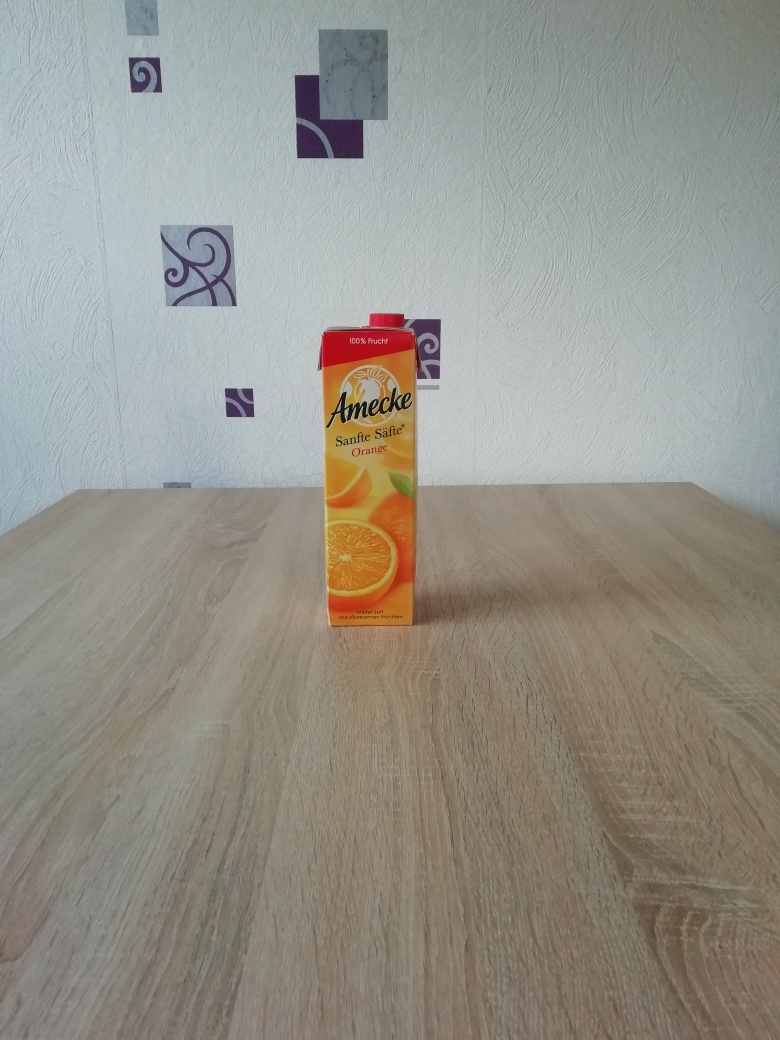
\includegraphics[width=\textwidth]{Sources/Bild1.jpg}
\end{minipage}
\hfill
\begin{minipage}[c]{0.08\textwidth}

\includegraphics[width=\textwidth]{Sources/Bild1.png}
\end{minipage}
\hfill
\begin{minipage}[c]{0.3\textwidth}
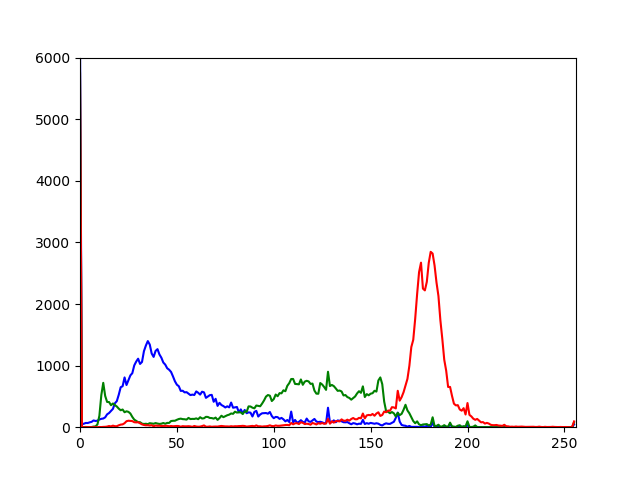
\includegraphics[width=\textwidth]{Sources/Bild1_histo.png}
\end{minipage}
\end{figure}
\begin{figure}[htb]
\begin{minipage}[c]{0.2\textwidth}
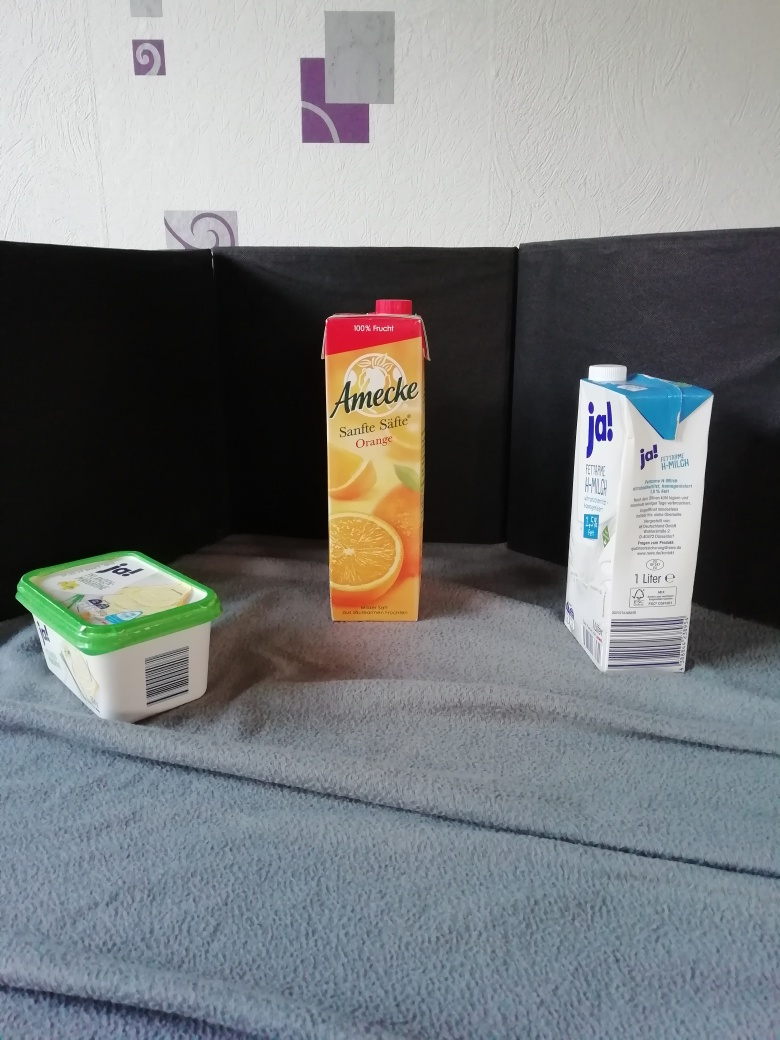
\includegraphics[width=\textwidth]{Sources/Bild2.jpg}
\end{minipage}
\hfill
\begin{minipage}[c]{0.08\textwidth}

\includegraphics[width=\textwidth]{Sources/Bild2.png}
\end{minipage}
\hfill
\begin{minipage}[c]{0.3\textwidth}
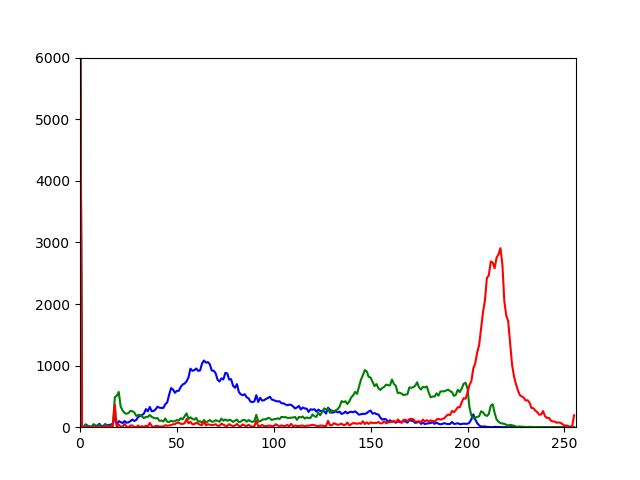
\includegraphics[width=\textwidth]{Sources/Bild2_histo.png}
\end{minipage}
\caption{Histogramm des Segmentierten Objektes aus dem Nahrungsmittel Datensatz. Ohne Normalisierung}
\label{img:evalnorm}
\end{figure}\\
Durch diesen Test wurde bestätigt, das die Ergebnisse der Histogramm Ausgleichung und Spezifikation sehr unterschiedlich geworden sind. Die Veränderung des Umfeldes beeinflusst also das Ergebnis entscheidend und sorgt für größere Farbveränderungen als der Lichteinfluss selbst.
Ein Datensatz mit einheitlichem Hintergrund in den Trainingsdaten, könnte mit den Normalisierungsverfahren besser funktionieren. Um diese Annahme weiter überprüfen zu können, soll ein weiterer Datensatz generiert werden, in welchem ein einheitlicher Hintergrund festgelegt ist. 
\section{Obst Datensatz}
Für einen weiteren Versuch, wurde der Obstdatensatz erstellt. Dieser besteht aus den Objekten welche in Tabelle \ref{tab:obst} aufgelistet sind. Bei diesem Datensatz wurde darauf geachtet einen einheitlichen Hintergrund zu verwenden, um die Funktionalität bei anderen Einstellungen zu testen. Außerdem wurde im Vergleich zum Nahrungsmittel Datensatz (Tabelle \ref{tab:nahrungsmittel}) darauf geachtet, ähnlichere Kassen zu verwenden, auf welchen optimaler Weise keine Schrift enthalten ist. Das Netz soll nicht durch die Schrift beeinflusst werden, sondern hauptsächlich die Farben als Orientierung nehmen.
\begin{table}[htb]
\caption{Klassen des Obst Datensatzes mit konstantem Hintergrund}
\center
\begin{minipage}[c]{.4\textwidth} 
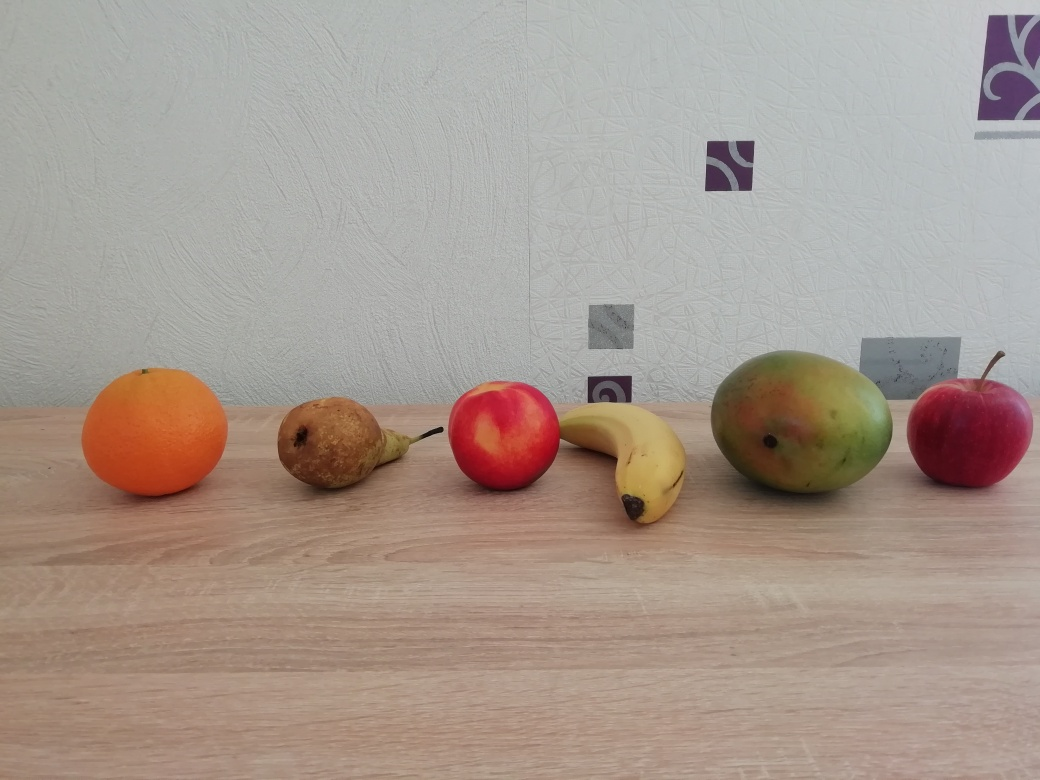
\includegraphics[width=.8\textwidth]{Sources/Obst_mit_hintergrund}  
\end{minipage} 
\begin{minipage}[c]{.4\textwidth}\label{tab:obst}   
\begin{tabular}{|l|l|}
\hline
Klassenname & Klassenname\\
\hline
Orange & Mango\\
Banane & Nektarine\\
Apfel & Birne\\
\hline
\end{tabular} 
\end{minipage}
\end{table}  
Dieser Datensatz wird nun genau wie die vorherigen Datensätze, mit den unterschiedlichen Methoden Normalisiert. Dabei soll zum einen die Genauigkeit der einzelnen Klassen betrachtet werden, zum anderen die Trainingsdaten an sich. Dabei soll überprüft werden, ob die Trainingsbilder wie erwartet aussehen und wie stark Anomalien auftreten. 
\section{Auswertung des Obst Datensatzes}
Nach Auswertung der Trainingsergebnisse kann festgestellt werden, das zwei der drein Normalisierungsmethoden einen positiven Einfluss auf die Klassifizierung haben. Die Genauigkeit der Histogramm Spezifikation schneidet mit 97\% am besten ab. Durch diese Methode konnte eine Erhöhung von 43\% erzielt werden. Auch der Gray-World-Algorithmus hat eine leichte Verbesserung von 14\% bewirkt. Lediglich der Histogramm Ausgleich hat die Klassifizierung leicht verschlechtert. Eine weitere Möglichkeit den Einfluss zu überprüfen, wurde mit Hilfe besonders schwierigen Testbildern versucht. Dafür sollen Bildaufnahmen bei extremen unterschiedlichen Lichteinflüssen verwendet werden.
\begin{table}
[h]
\caption{Genauigkeitsberechnungen des Modells des Obst Datensatzes}
\centering
\begin{tabular}{|l|c|c|c|c|}
\hline
Klassenname & AP(N) & AP(GW) & AP(HA) & AP(HS)\\
\hline
Orange & \textcolor{red}{0.982} & 0.985 & 0.983 & \textcolor{green}{1.000}\\
Nektarine & \textcolor{red}{0.986} & 0.988 & \textcolor{green}{0.993} & 0.987\\
Banane & \textcolor{green}{1.000} & \textcolor{green}{1.000} & \textcolor{green}{1.000} & \textcolor{green}{1.000}\\
Mango & 0.993 & 0.996 & \textcolor{red}{0.983} & \textcolor{green}{1.000}\\
Apfel & 0.995 & 0.996 & \textcolor{red}{0.990} & \textcolor{green}{0.999}\\
Birne & 0.999 & \textcolor{red}{0.998} & \textcolor{green}{1.000} & \textcolor{green}{1.000}\\
\hline
mAP & 0.993 & 0.994 & \textcolor{red}{0.992} & \textcolor{green}{0.997}\\
\hline
\end{tabular}
\end{table}
Die Auswertung der normalisierten Trainingsdaten hat ergeben, das wesentlich weniger farb-Anomalien auftreten, wie bei den vorherigen Datensätzen. Dabei ist aufgefallen das gerade bei den Histogramm Normalisierungen mit einheitlichen Hintergrund deutliche Verbesserungen erzielt wurden. Große Veränderungen treten nur dann auf, wenn viele Objekte auf dem Bild enthalten sind, da diese die Umgebung zu stark beeinflussen oder bei der Histogramm Ausgleichung, wenn die Beleuchtungen zu extrem verändert wurde. Die Histogramm Spezifikation geht mit diesem Problem noch am besten um, weil diese ein Referenz-Histogramm verwendet, um die Daten anzupassen. \\\\
Auch eine Betrachtung der Helligkeitsverteilung der Trainingsdaten werden wesentlich besser wie in den Beispielen in Abbildung \ref{img:hellver} zu erkennen ist. Dafür wurde eine stark unterbelichtete Aufnahme generiert, um die Veränderung nach den Normalisierungsmethoden besser herauszustellen. Die beste Helligkeitsverteilung konnte dabei der Histogramm Ausgleich aufweisen, wobei durch das dunkle Quellbild die Farbinformationen zum großen Teil verloren gegangen sind. Der Gray World hat die Helligkeitsverteilung kaum verändert, was aber daran liegt, dass die Farbverteilung durch die Höhe des Grün Kanals verschoben wird und nicht für solche Aufgaben ausgelegt ist. Das insgesamt beste Ergebnis liefert die Histogramm Spezifikation. Nicht nur die Helligkeitsverteilung konnte verbessert werden, auch die Farben konnten vergleichsweise gut wieder hergestellt werden.
	
% Die Zähler für Tabellen und Abbildungen werden zurückgesetzt, damit
	% in jedem Kapitel die Nummerierung neu beginnt
\setcounter{table}{1}
\setcounter{figure}{1}
	% Einbinden des dritten Kapitels
	%!TEX root = ../draft.tex
\chapter{Diskussion}\label{s.diskussion}
In diesem Kapitel sollen die Ergebnisse und Erkenntnisse, welche im Verlauf der Arbeit herausgearbeitet wurden, kurz aufgeführt und erläutert werden.
\section{Datensätze und Netze}
Die Daten der trainierten Netze zeigen, dass mit den verwendeten Datensätzen und den angewandten Normalisierungsmethoden keine Erhöhung der Genauigkeit erzielt werden konnte. Ein möglicher Grund sind die Datensätze, welche normalisiert wurden. Da manche Normalisierungsverfahren die Farbinformationen des gesamten Bildes verwendeten, ist das Ergebnis der Normalisierungen, je nach Umgebung, in den Bildern unterschiedlich ausgefallen. Um diese Annahme zu überprüfen, wurden Testaufnahmen von Objekten auf verschiedenen Hintergründen mit gleicher Belichtung und gleichem Aufnahmewinkel erstellt. In den unveränderten Testbildern ist kein großer Unterschied in den Histogrammen aufgefallen. Bei gleicher Lichteinstrahlung und unterschiedlichen Hintergründen haben die Objekte eine fast identische Farbverteilung. Lediglich die Helligkeit hat etwas variiert. Der normalisierte Datensatz jedoch zeigt größere Unterschiede in den Histogrammen und bei den Farben. Das könnte daran liegen, dass die Normalisierung nicht nur die Objekte auf den Bildern normalisiert, sondern auch den Hintergrund, welcher bei vielen der Trainingsbilder unterschiedlich ist.\\ 
Die Überprüfung hat gezeigt, dass die Datensätze für den verwendeten Aufbau und den verwendeten Normalisierungsalgorithmen nicht geeignet waren. Bessere Ergebnisse konnten mit dem im nachhinein generierten Obst-Datensatz erzielt werden, bei dem alle Trainingsdaten auf demselben Hintergrund aufgenommen wurden. Dadurch konnten alle Klassen auf derselben Basis normalisiert werden. Gerade die Histogramm-Spezifikation (Abbildung \ref{img:hellver}) hat hier besonders gute Ergebnisse erzielt, da der Einsatz eines Referenzbildes besser funktioniert hat und wesentlich weniger Anomalien erzeugt wurden. Auch bei der Untersuchung der Helligkeit konnten wesentliche Verbesserungen festgestellt werden. Bei einem stark unterbelichteten Bild wurde, durch den Histogramm-Ausgleich, die Lichtverteilung wesentlich angehoben. Die Farbinformationen konnten jedoch größtenteils nicht wiederhergestellt werden. Durch die Histogramm-Spezifikation hat sich auch die Lichtverteilung verbessert und durch das Referenzbild wurden zudem die Farbinformationen wiederhergestellt. Der Gray-World-Algorithmus schneidet hier am schlechtesten ab, da dieser nicht mit den einzelnen Farbwerten arbeitet, sondern die gesamten Farbkanäle auf Basis des Grünkanals verschiebt und nur Lichtfarben ausgleicht. 
\section{Laufzeittest}
Ein weiterer Einfluss, welchen die Normalisierungsalgorithmen auf die Klassifizierung von neuronalen Netzen haben, ist, neben dem Manipulieren von Trainingsdaten, die Zeit welche das jeweilige Verfahren benötigt. Um herauszufinden, wie sich die Laufzeit bei größer werdenden Bilddateien verhält, wurde ein Bild in verschiedenen Größen getestet.
\begin{table}
[h]
\caption{Laufzeiten der Normalisierungs-Algorithmen mit verschieden großen Bildern}
\centering
\begin{tabular}{|l|c|c|c|c|c|}
\hline
Bildgröße & Faktor & Dateigröße & GW(s) & HA(s) & HS(s)\\
\hline
4160x3120 & 100\% & 2.441 KB & 1,447s & 0,172s & 6,952s\\
2912x2184 & 70\% & 1.000 KB & 0,755s & 0,078s & 3,215s\\
2080x1560 & 50\% & 529 KB & 0,362s & 0,035s & 1,717s\\
1040x780 & 25\% & 114 KB & 0,094s & 0,013s & 0,422s\\
\hline
\end{tabular}
\end{table}
Der Gray-World-Algorithmus liegt, im Vergleich zu den anderen Methoden, bei der Laufzeit im Mittelfeld. Bei Verdoppelung der Bildgröße erhöht sich die Laufzeit um das Vierfache. Dabei sind sowohl die Farbgebung, als auch der Kontrast nicht entscheidend. Die Histogramm-Ausgleichung ist in diesem Fall die schnellste Methode, wobei hierbei die Verteilung im Histogramm eine Rolle spielt. Die Laufzeit verändert sich nicht linear, sondern steigt exponentiell an. So steigt die Laufzeit beim Verdoppeln um den Faktor drei und beim nächsten Mal um den Faktor sechs. Der längste Normalisierungsalgorithmus ist in diesem Fall die Histogramm-Spezifikation. Dabei spielt die Größe des Referenzbildes eine wichtige Rolle. Mit einem größeren Referenzbild würde sich die Laufzeit noch weiter erhöhen. Bei einem gleichbleibenden Referenzbild erhöht sich die Laufzeit um den Faktor vier. Durch die hohe Grundlaufzeit führt das schnell zu langen Laufzeiten. Hierbei muss beachtet werden, dass die Laufzeiten nur für ein Bild berechnet wurden. Für ein künstliches neuronales Netz werden meist mehrere Tausend Bilder verwendet. Hier muss, je nach Datensatz, abgewägt werden, ob die erhöhte Laufzeit für eine Normalisierung in Kauf genommen werden soll.

	
	% Die Zähler für Tabellen und Abbildungen werden zurückgesetzt, damit
	% in jedem Kapitel die Nummerierung neu beginnt
\setcounter{table}{1}
\setcounter{figure}{1}
	% Einbinden des dritten Kapitels
	%!TEX root = ../draft.tex
\chapter{Fazit}\label{s.fazit}
Zunächst wird auf die Anforderungen eingegangen und wie gut diese erfüllt werden konnten. Für ein abschließendes Fazit wird anschließend erläutert auf welche Art von Datensätzen, die in dieser Arbeit untersuchten Normalisierungsverfahren angewendet werden können und wo die Schwächen liegen.\\\\
Bei der ersten Anforderung ging es um das Training des neuronalen Netzes und um eine Möglichkeit mit weniger Bildern pro Datensatz auszukommen. Dieser Punkt konnte erfüllt werden, indem vortrainierte künstliche neuronale Netze verwendet wurden. Dadurch sind die Mengen der Trainingsdaten auf durchschnittlich 200 Bilder pro Klasse gesunken.\\\\
Bei den Anforderungen zwei bis fünf wurden die Datensätze, welche bei dem Versuch verwendet werden sollten, spezifiziert. Die Anforderung zwei, bei der es um die Ordentlichkeit der Datensätze geht, konnte nicht bei jedem Datensatz erfüllt werden. Der PascalVOC-Datensatz hat die Trainingsdaten gemischt und erschwerte dadurch das Verändern der einzelnen Klassen. Die dritte Anforderung, in der es um die Größe der Bilder ging, wurde bei jedem Datensatz erfüllt. Die Bilder haben eine Größe zwischen 100-300 KB. Anforderung vier, in der es um die Ausleuchtung der Trainingsdaten ging, wurde nur teilweise erfüllt, da für das Testen der neuronalen Netze auch schlecht ausgeleuchtete Testdaten benötigt wurden. Bei Anforderung fünf ging es um die Definition eines eingegrenzten Themas, der einzelnen Datensätze. Jeder Datensatz hatte ein gut definiertes Thema, welches unter anderem sehr ähnliche Klassen besaß. Beim PascalVOC-Datensatz war dieser teilweise ziemlich willkürlich, hat aber in der Klassifizierung relativ gut funktioniert.\\\\
Bei der Anforderungen sechs ging es um die Anwendung der Normalisierungsverfahren auf verschiedene Datensätze. Dabei sollte herausgestellt werden, ob und unter welchen Bedingungen eine Farbnormalisierung einen positiven Einfluss, auf eine Klassifizierung durch neuronale Netze, hat. Dabei sind je nach Normalisierungsverfahren unterschiedliche Ergebnisse entstanden, welche im Folgenden nacheinander behandelt werden.\\\\
\textbf{Gray-World-Algorithmus}\\
Der Gray-World-Algorithmus kann prinzipiell bei jedem Datensatz angewendet werden. Der Vorteil wird deutlich, wenn verschiedene Lichtfarben in der späteren Erkennung und im Datensatz auftauchen. Durch diese Methode werden Kontrast und Dynamik nicht verändert. Das Farbbild wird insgesamt auf Grundlage des Grünkanals verschoben. Da dieses Verfahren relativ simpel arbeitet, wird kein großer Einfluss auf spätere künstliche neuronale Netze erzielt.\\\\
\textbf{Histogramm-Ausgleich}\\
Der Histogramm-Ausgleich arbeitet auf Grundlage des Histogramms und versucht den Kontrast in dem Bild zu erhöhen. Eingesetzt werden kann es bei Datensätzen, welche einen einheitlichen Hintergrund verwenden, da für die Normalisierung die Farbverteilung des gesamten Bildes verwendet wird. Denn je nach Farbverteilung fällt das Ausgabebild, nach dem Ausgleich, unterschiedlich aus. Schwächen gibt es bei starken Lichtunterschieden. Sollte ein Bild zu dunkel sein, können Farbwerte nicht wiederhergestellt werden.\\\\
\textbf{Histogramm-Spezifizierung}\\
Auch die Histogramm-Spezifizierung ist nicht für allgemeine Datensätze geeignet, sondern für Datensätze mit einheitlichem Hintergrund. Das liegt zum einen an der Verarbeitung des Histogramms und zum anderen an der Tatsache, dass für dieses Verfahren ein Referenzbild benötigt wird, auf welchem der Datensatz normalisiert wird. Dieses Referenzbild ist effektiver, desto ähnlicher es dem Datensatz ist. Die Ergebnisse dieses Verfahrens haben beim Obst-Datensatz eine deutlich erhöhte Genauigkeit erzielt. Bei diesem Verfahren muss beachtet werden, dass es die längste Laufzeit hat und eine gewisse Arbeit voraussetzt.\\\\
In dieser Arbeit sollte überprüft werden, ob die Anwendung von Farbnormalisierungsalgorithmen einen positiven Einfluss auf die Genauigkeit der Klassifizierung, mittels künstliche neuronaler Netze, haben. Dabei ist herausgekommen, dass Farbnormalisierung einen positiven Einfluss haben kann. Wichtig dabei ist auf die Funktionsweise der Verfahren zu achten und zu prüfen für welche Szenarien diese sinnvoll eingesetzt werden können. Dafür ist es in manchen Fällen notwendig, die Datensätze an die Normalisierungen anzupassen.\\\\
Im  weiteren sollen Ansätze aufgeführt werden, die die Forschung nach dieser Arbeit weiter verfolgen kann. In dieser Arbeit wurden die Verfahren mit vortrainierten neuronalen Netzen überprüft. Es wäre daher eine interessante Frage, wie im Vergleich dazu untrainierte neuronale Netze die Verfahren beeinflussen. Zudem konnten im Rahmen dieser Bachelorarbeit nur Datensätze in der Mindestgröße generiert werden. Deswegen wäre es ebenso spannend herauszufinden, wie die Ergebnisse bei wesentlich größeren und ausführlicheren Datensätzen aussehen würden.\\
Außerdem könnte das Verhalten der Normalisierungsmethoden in Kombination miteinander untersucht werden. Möglicherweise können durch solche Kombinationen die unterschiedlichen Stärken der Verfahren zusammen genutzt werden.  


\singlespacing
%!TEX root = ../draft.tex

  
  	%Erzeugt ein Abbildungsverzeichnis
	\listoffigures
	%Fügt die Zeile "`Abbildungsverzeichnis"' als Chapter ins Inhaltsverzeichnis ein
	\addcontentsline{toc}{chapter}{Abbildungsverzeichnis}
	
	%Erzeugt ein Tabellenverzeichnis
	\listoftables
	%Fügt die Zeile "`Tabellenverzeichnis"' als Chapter ins Inhaltsverzeichnis ein
	\addcontentsline{toc}{chapter}{Tabellenverzeichnis}
	
	%Ändert den Stil des Literaturverzeichnisses
	%\bibliographystyle{alpha}
	%Erzeugt das Literaturverzeichnis anhand der Datei "`literatur.bib"'
	\bibliography{literatur}
	%Fügt die Zeile "`Literaturverzeichnis"' als Chapter ins Inhaltsverzeichnis ein
	\addcontentsline{toc}{chapter}{Literaturverzeichnis}
  
  	
\nocite{*}

%=== Schlussteil =====================================================
\backmatter
\pagenumbering{Roman}

\setcounter{table}{1}
\setcounter{figure}{1}
%!TEX root = ../draft.tex

\begin{appendices}
% \adjustmtc 
\renewcommand{\appendixname}{ANHANG}
\renewcommand{\appendixtocname}{\appendixname} 
\addappheadtotoc 

% \begin{mtchideinmaintoc}[0]   %  [-1] Den folgenden Inhalt nicht im großen Inhaltsverzeichnis zeigen, [0] ab Chapter im großen Inhaltsverzeichnis anzeigen

\part*{Anhang}
\begin{figure}[htb]
\begin{minipage}[c]{0.2\textwidth}
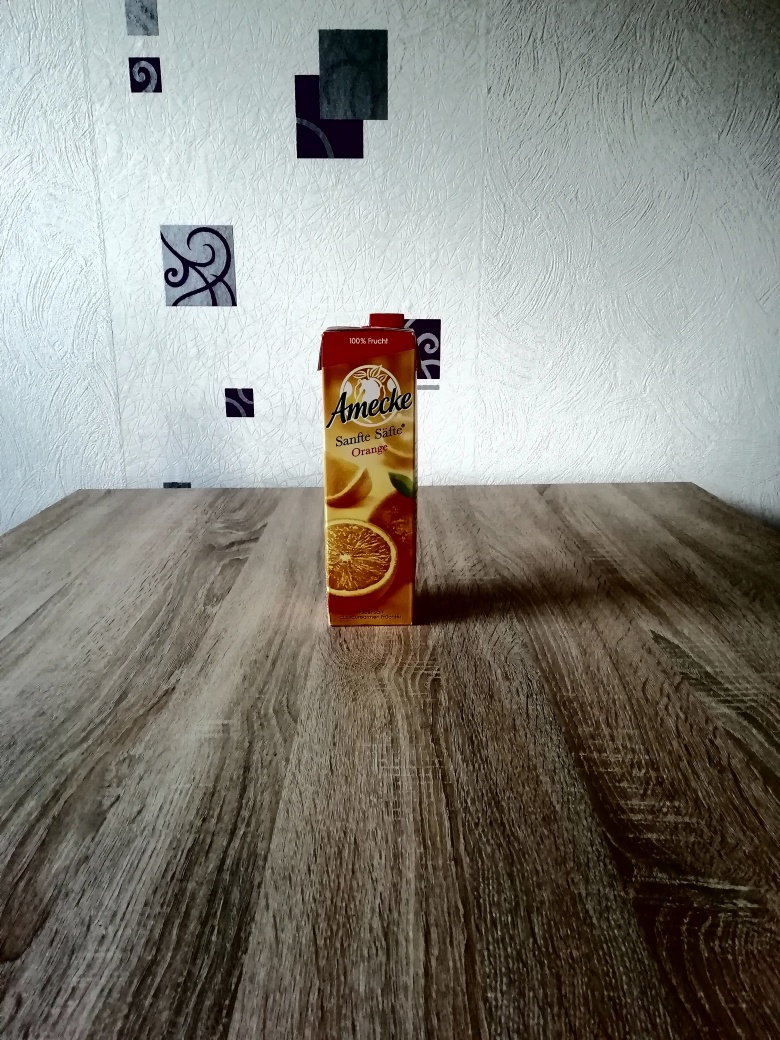
\includegraphics[width=\textwidth]{Sources/Bild1_HA.jpg}
\end{minipage}
\hfill
\begin{minipage}[c]{0.08\textwidth}

\includegraphics[width=\textwidth]{Sources/Bild1_HA.png}
\end{minipage}
\hfill
\begin{minipage}[c]{0.3\textwidth}
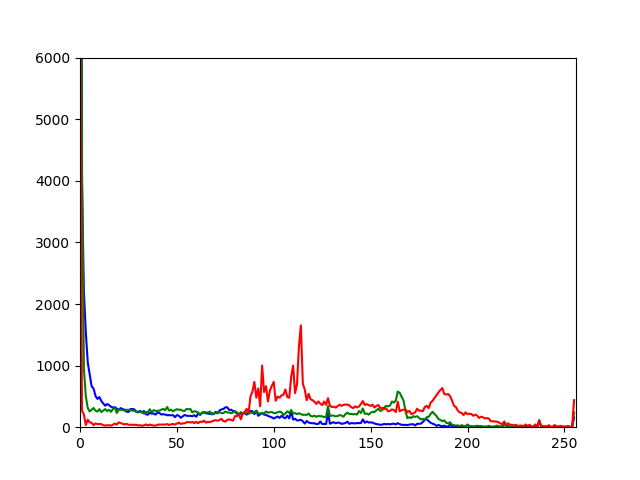
\includegraphics[width=\textwidth]{Sources/Bild1_HA_histo.png}
\end{minipage}
\end{figure}
\begin{figure}[htb]
\begin{minipage}[c]{0.2\textwidth}
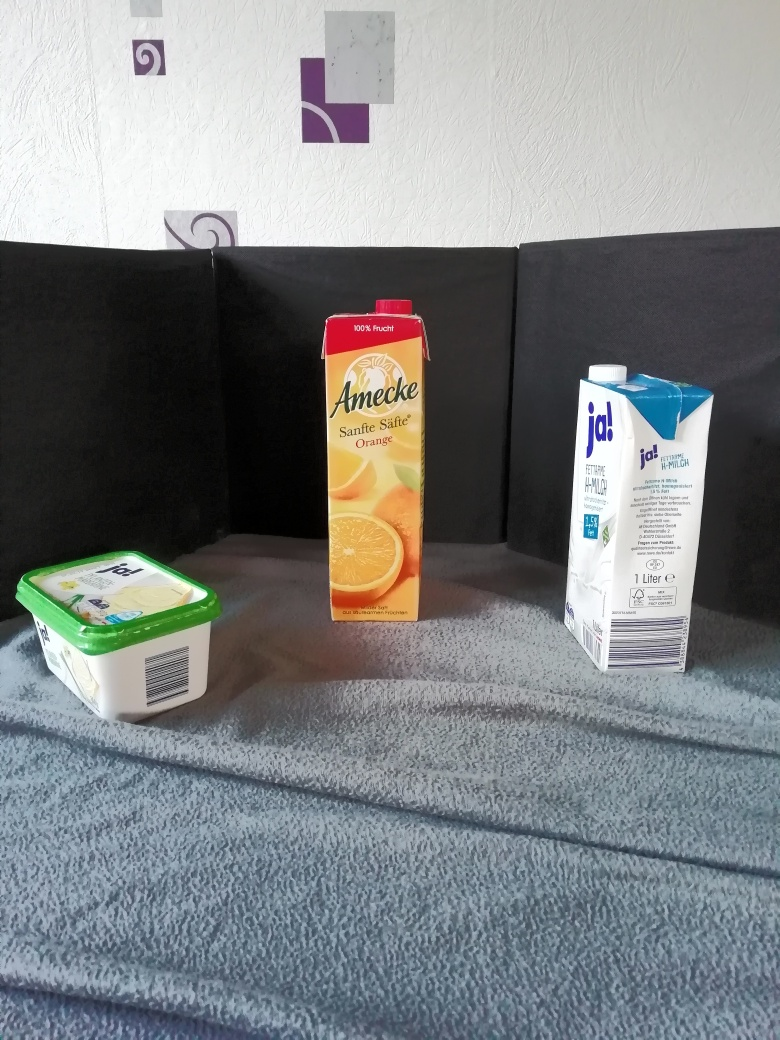
\includegraphics[width=\textwidth]{Sources/Bild2_HA.jpg}
\end{minipage}
\hfill
\begin{minipage}[c]{0.08\textwidth}

\includegraphics[width=\textwidth]{Sources/Bild2_HA.png}
\end{minipage}
\hfill
\begin{minipage}[c]{0.3\textwidth}
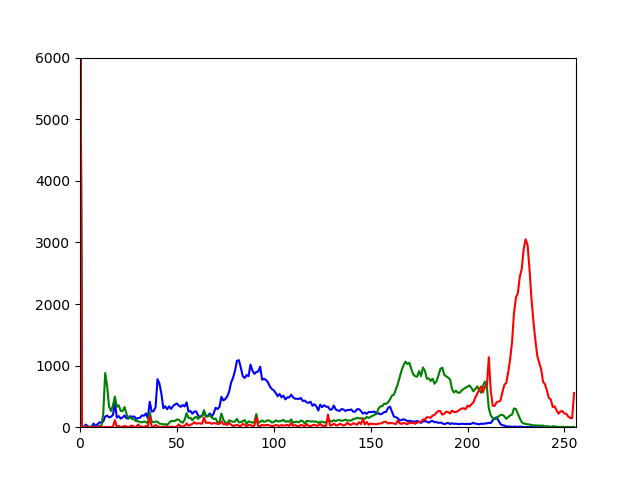
\includegraphics[width=\textwidth]{Sources/Bild2_HA_histo.png}
\end{minipage}
\end{figure}
\begin{figure}[htb]
\begin{minipage}[c]{0.2\textwidth}
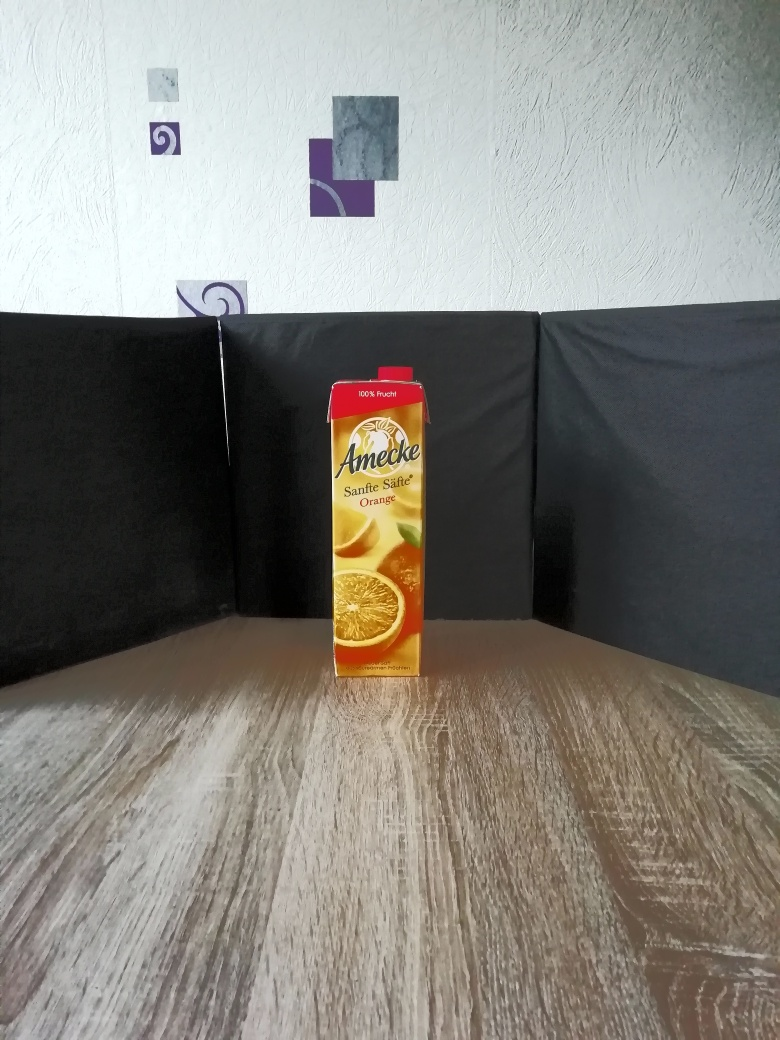
\includegraphics[width=\textwidth]{Sources/Bild3_HA.jpg}
\end{minipage}
\hfill
\begin{minipage}[c]{0.08\textwidth}

\includegraphics[width=\textwidth]{Sources/Bild3_HA.png}
\end{minipage}
\hfill
\begin{minipage}[c]{0.3\textwidth}
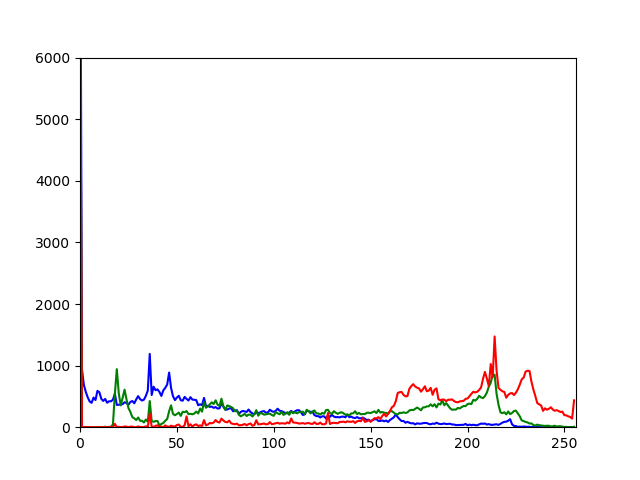
\includegraphics[width=\textwidth]{Sources/Bild3_HA_histo.png}
\end{minipage}
\caption{Histogramm des segmentierten Objektes aus dem Nahrungsmittel-Datensatz. Normalisiert durch den Histogramm-Ausgleich}
\label{img:evalHA}
\end{figure}
\newpage
\begin{figure}[htb]
\begin{minipage}[c]{0.2\textwidth}
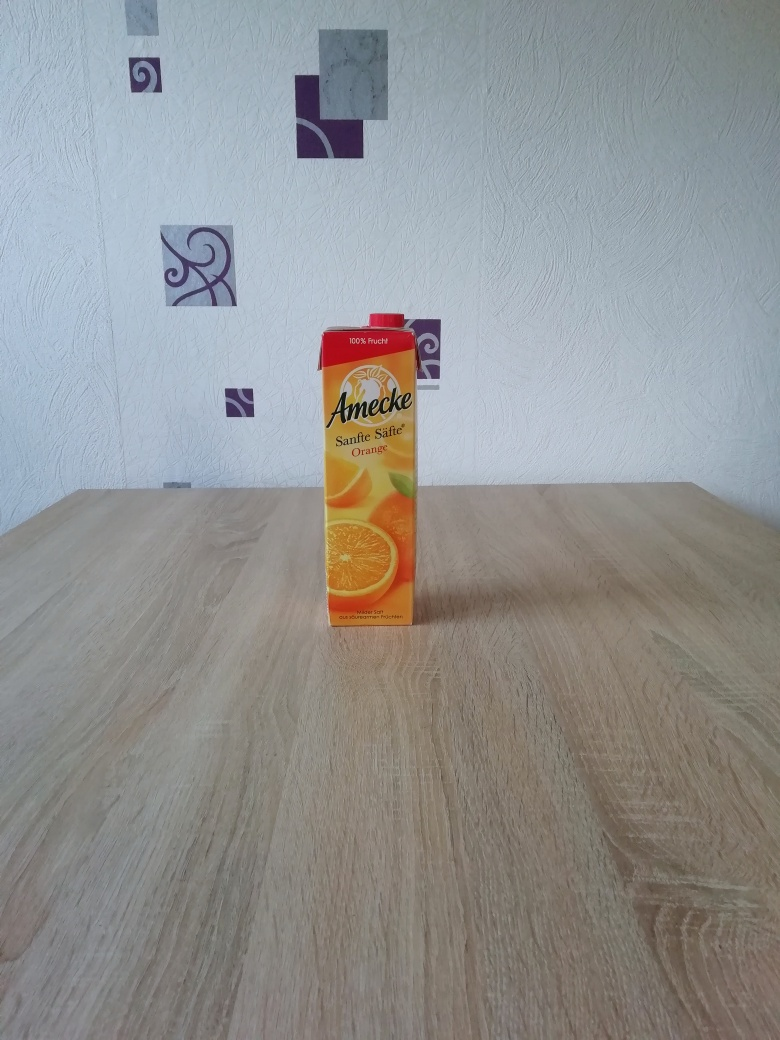
\includegraphics[width=\textwidth]{Sources/Bild1_GW.jpg}
\end{minipage}
\hfill
\begin{minipage}[c]{0.08\textwidth}

\includegraphics[width=\textwidth]{Sources/Bild1_GW.png}
\end{minipage}
\hfill
\begin{minipage}[c]{0.3\textwidth}
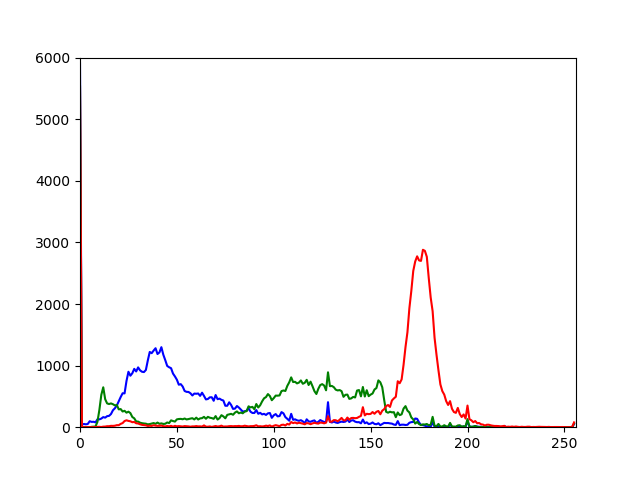
\includegraphics[width=\textwidth]{Sources/Bild1_GW_histo.png}
\end{minipage}
\end{figure}
\begin{figure}[htb]
\begin{minipage}[c]{0.2\textwidth}
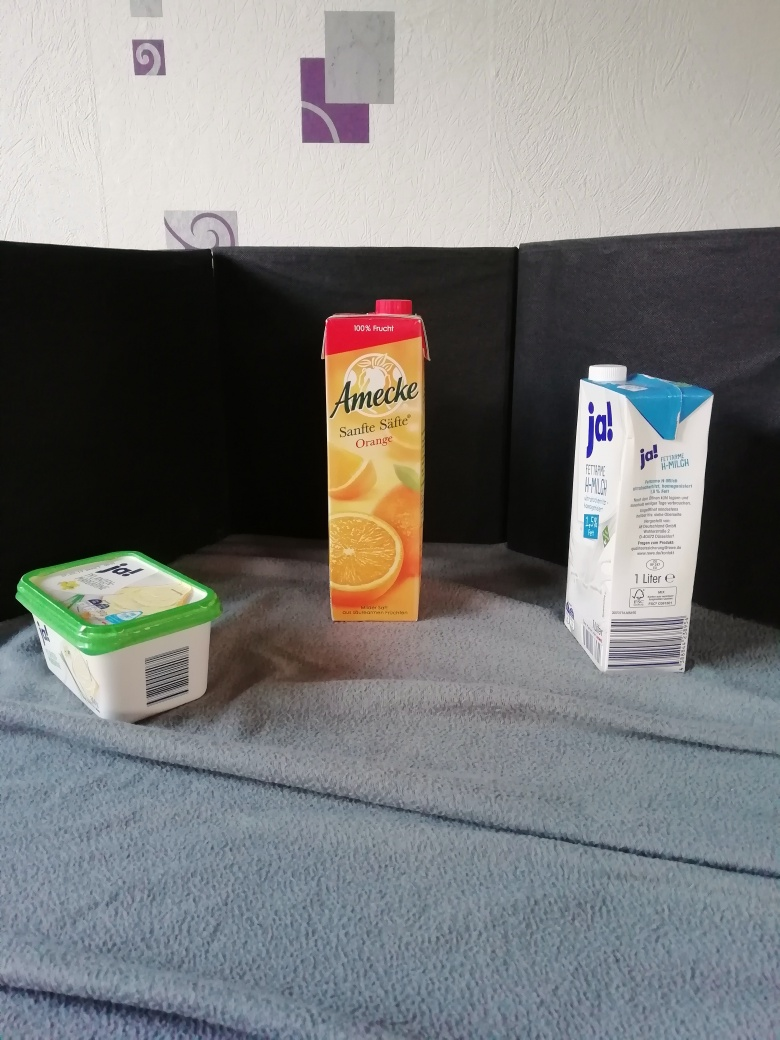
\includegraphics[width=\textwidth]{Sources/Bild2_GW.jpg}
\end{minipage}
\hfill
\begin{minipage}[c]{0.08\textwidth}

\includegraphics[width=\textwidth]{Sources/Bild2_GW.png}
\end{minipage}
\hfill
\begin{minipage}[c]{0.3\textwidth}
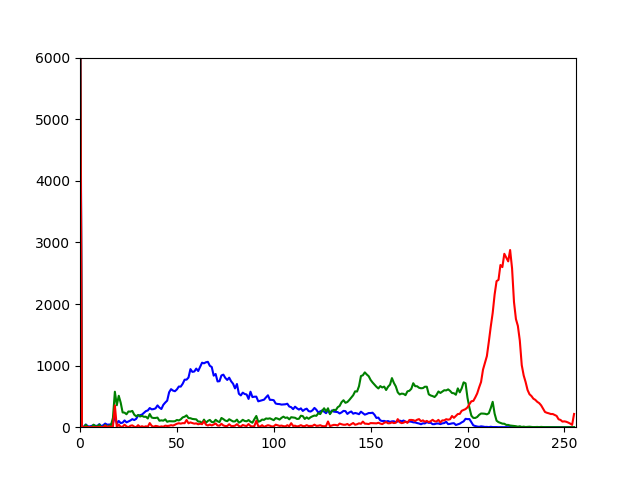
\includegraphics[width=\textwidth]{Sources/Bild2_GW_histo.png}
\end{minipage}
\end{figure}
\begin{figure}[htb]
\begin{minipage}[c]{0.2\textwidth}
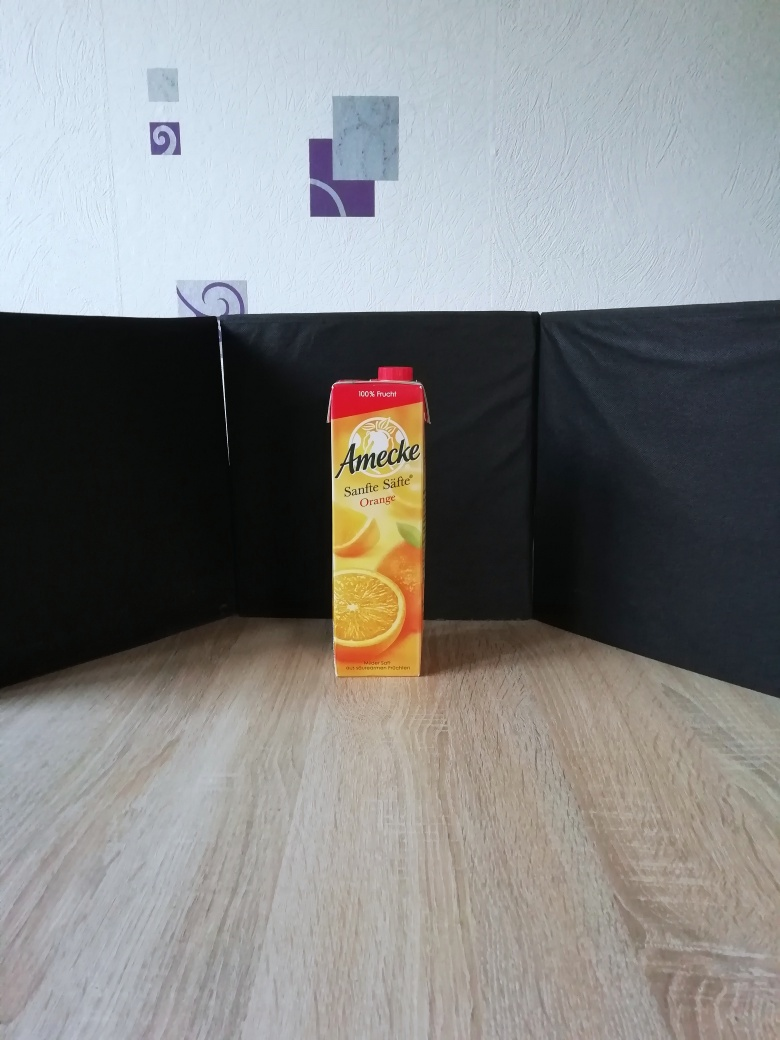
\includegraphics[width=\textwidth]{Sources/Bild3_GW.jpg}
\end{minipage}
\hfill
\begin{minipage}[c]{0.08\textwidth}

\includegraphics[width=\textwidth]{Sources/Bild3_GW.png}
\end{minipage}
\hfill
\begin{minipage}[c]{0.3\textwidth}
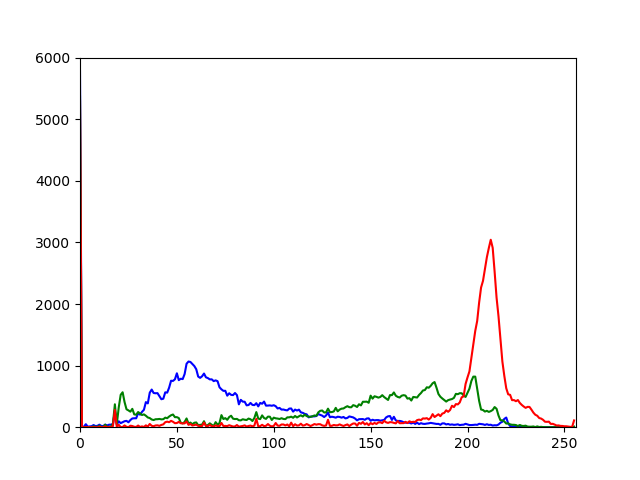
\includegraphics[width=\textwidth]{Sources/Bild3_GW_histo.png}
\end{minipage}
\caption{Histogramm des segmentierten Objektes aus dem Nahrungsmittel-Datensatz. Normalisiert durch den Gray-World-Algorithmus}
\label{img:evalGW}
\end{figure}
\newpage
\begin{figure}[htb]
\begin{minipage}[c]{0.2\textwidth}
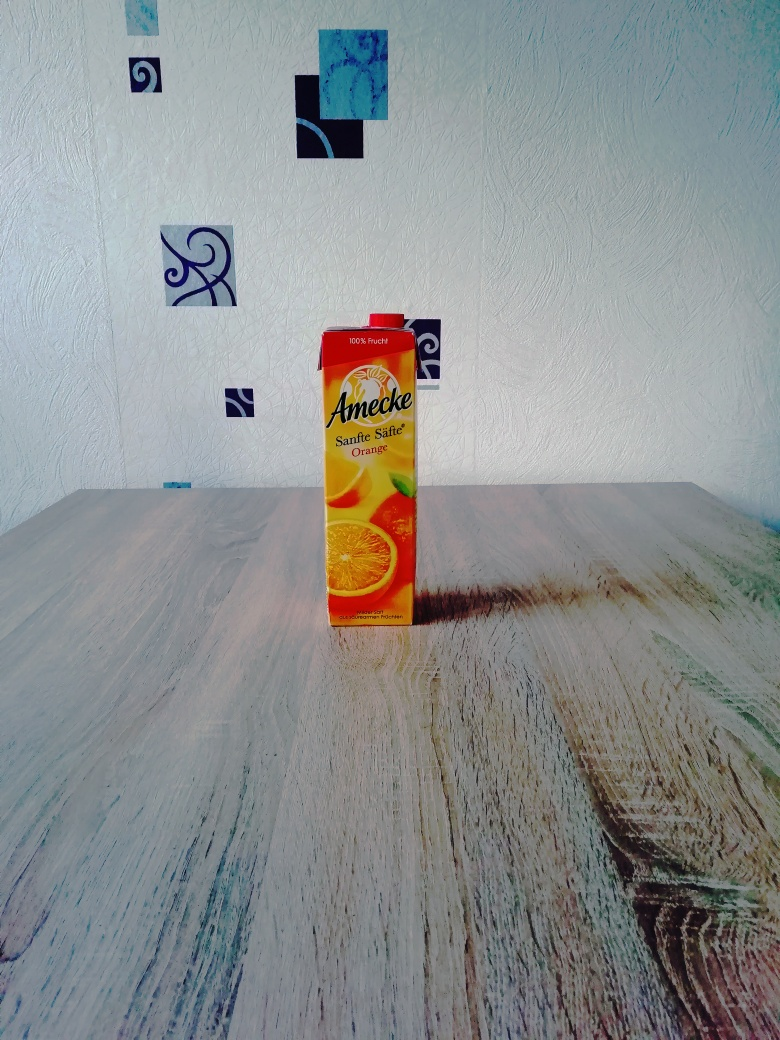
\includegraphics[width=\textwidth]{Sources/Bild1_HS.jpg}
\end{minipage}
\hfill
\begin{minipage}[c]{0.08\textwidth}

\includegraphics[width=\textwidth]{Sources/Bild1_HS.png}
\end{minipage}
\hfill
\begin{minipage}[c]{0.3\textwidth}
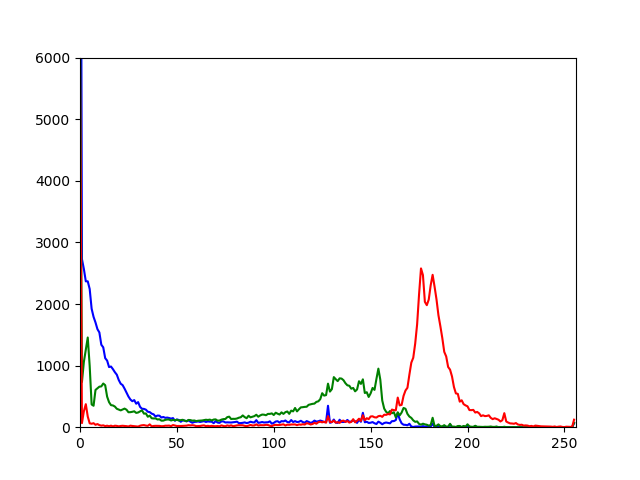
\includegraphics[width=\textwidth]{Sources/Bild1_HS_histo.png}
\end{minipage}
\end{figure}
\begin{figure}[htb]
\begin{minipage}[c]{0.2\textwidth}
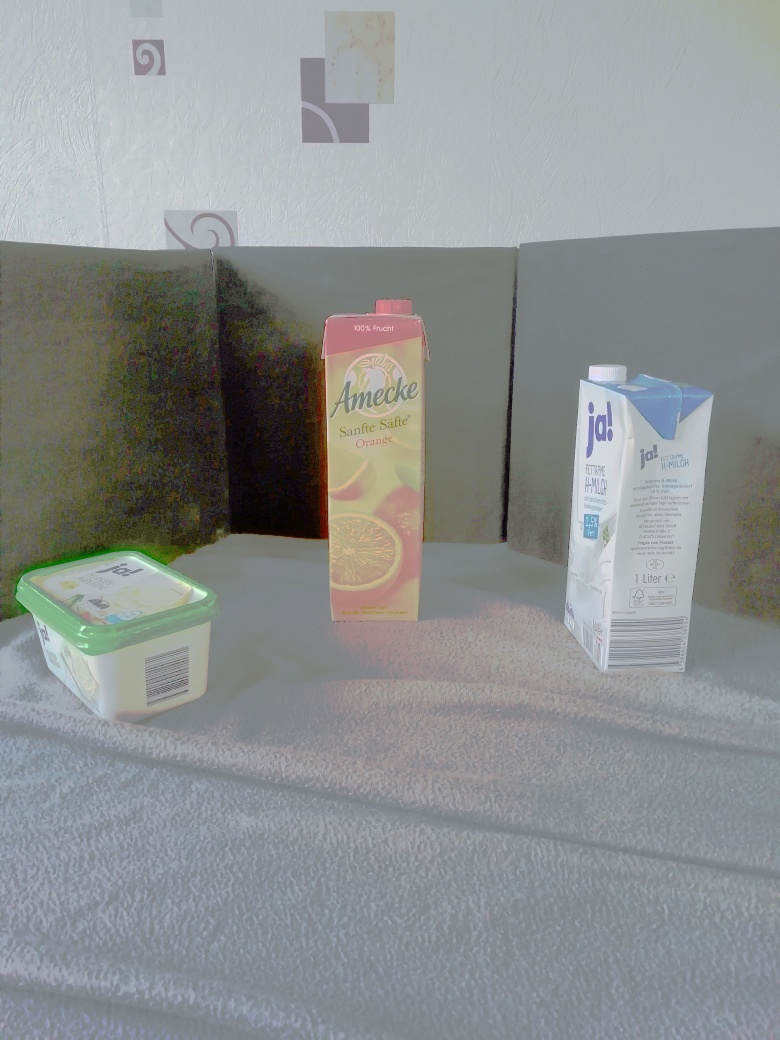
\includegraphics[width=\textwidth]{Sources/Bild2_HS.jpg}
\end{minipage}
\hfill
\begin{minipage}[c]{0.08\textwidth}
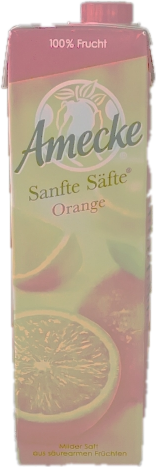
\includegraphics[width=\textwidth]{Sources/Bild2_HS.png}
\end{minipage}
\hfill
\begin{minipage}[c]{0.3\textwidth}
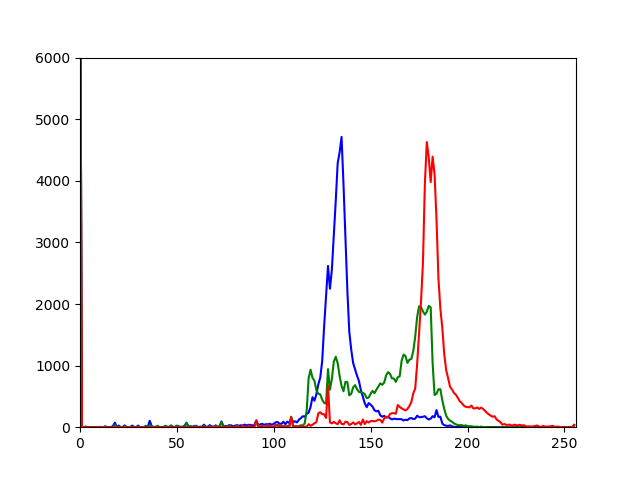
\includegraphics[width=\textwidth]{Sources/Bild2_HS_histo.png}
\end{minipage}
\end{figure}
\begin{figure}[htb]
\begin{minipage}[c]{0.2\textwidth}
\includegraphics[width=\textwidth]{Sources/Bild3_HS.jpg}
\end{minipage}
\hfill
\begin{minipage}[c]{0.08\textwidth}
\includegraphics[width=\textwidth]{Sources/Bild3_HS.png}
\end{minipage}
\hfill
\begin{minipage}[c]{0.3\textwidth}
\includegraphics[width=\textwidth]{Sources/Bild3_HS_histo.png}
\end{minipage}
\caption{Histogramm des segmentierten Objektes aus dem Nahrungsmittel-Datensatz. Normalisiert durch die Histogramm-Spezifikation}
\label{img:evalHS}
\end{figure}
\begin{figure}[htbp]
\center
\begin{minipage}{0.49\textwidth}
\includegraphics[width=.8\textwidth]{Sources/Anhang/resize_0250.jpg}
\end{minipage}
\begin{minipage}{0.49\textwidth}
\includegraphics[width=\textwidth]{Sources/Anhang/resize_0250.png}
\end{minipage}
\begin{minipage}{0.49\textwidth}
\includegraphics[width=.8\textwidth]{Sources/Anhang/resize_0250_GW.jpg}
\end{minipage}
\begin{minipage}{0.49\textwidth}
\includegraphics[width=\textwidth]{Sources/Anhang/resize_0250_GW.png}
\end{minipage}
\begin{minipage}{0.49\textwidth}
\includegraphics[width=.8\textwidth]{Sources/Anhang/resize_0250_HA.jpg}
\end{minipage}
\begin{minipage}{0.49\textwidth}
\includegraphics[width=\textwidth]{Sources/Anhang/resize_0250_HA.png}
\end{minipage}
\begin{minipage}{0.49\textwidth}
\includegraphics[width=.8\textwidth]{Sources/Anhang/resize_0250_HS.jpg}
\end{minipage}
\begin{minipage}{0.49\textwidth}
\includegraphics[width=\textwidth]{Sources/Anhang/resize_0250_HS.png}
\end{minipage}
\caption{Helligkeitsverteilung und der Einfluss der Normalisierungs-Algorithmen auf das Testbild}
\label{img:hellver}
\end{figure}

\begin{figure}[htb]
\center
\begin{minipage}{0.19\textwidth}
\includegraphics[width=\textwidth]{images/anomalien/HA/000613.jpg}
\end{minipage}
\begin{minipage}{0.19\textwidth}
\includegraphics[width=\textwidth]{images/anomalien/HA/000750.jpg}
\end{minipage}
\begin{minipage}{0.19\textwidth}
\includegraphics[width=\textwidth]{images/anomalien/HA/000777.jpg}
\end{minipage}
\begin{minipage}{0.19\textwidth}
\includegraphics[width=\textwidth]{images/anomalien/HA/001608.jpg}
\end{minipage}
\begin{minipage}{0.19\textwidth}
\includegraphics[width=\textwidth]{images/anomalien/HA/003339.jpg}
\end{minipage}
\begin{minipage}{\textwidth}
\hspace{\textwidth}
\end{minipage}
\begin{minipage}{0.19\textwidth}
\includegraphics[width=\textwidth]{images/anomalien/HA/image41.jpg}
\end{minipage}
\begin{minipage}{0.19\textwidth}
\includegraphics[width=\textwidth]{images/anomalien/HA/image67.jpg}
\end{minipage}
\begin{minipage}{0.19\textwidth}
\includegraphics[width=\textwidth]{images/anomalien/HA/image104.jpg}
\end{minipage}
\begin{minipage}{0.19\textwidth}
\includegraphics[width=\textwidth]{images/anomalien/HA/image157.jpg}
\end{minipage}
\begin{minipage}{0.19\textwidth}
\includegraphics[width=\textwidth]{images/anomalien/HA/IMG_20181209_160502.jpg}
\end{minipage}
\begin{minipage}{\textwidth}
\hspace{\textwidth}
\end{minipage}
\begin{minipage}{0.19\textwidth}
\includegraphics[width=\textwidth]{images/anomalien/HA/n02085620_952.jpg}
\end{minipage}
\begin{minipage}{0.19\textwidth}
\includegraphics[width=.8\textwidth]{images/anomalien/HA/n02088466_9359.jpg}
\end{minipage}
\begin{minipage}{0.19\textwidth}
\includegraphics[width=\textwidth]{images/anomalien/HA/n02088466_9691.jpg}
\end{minipage}
\begin{minipage}{0.19\textwidth}
\includegraphics[width=\textwidth]{images/anomalien/HA/n02089078_4544.jpg}
\end{minipage}
\begin{minipage}{0.19\textwidth}
\includegraphics[width=\textwidth]{images/anomalien/HA/n02091032_12113.jpg}
\end{minipage}
\caption{Auftretende Farbanomalien in den drei Datensätzen durch den Histogramm-Ausgleich. Oben: PascalVOC-Datensatz, Mitte: Nahrungsmittel-Datensatz, Unten: Stanford Dog-Datensatz}
\label{img:anoHA}
\end{figure}

\begin{figure}[htb]
\center
\begin{minipage}{0.19\textwidth}
\includegraphics[width=\textwidth]{images/anomalien/HS/007911.jpg}
\end{minipage}
\begin{minipage}{0.19\textwidth}
\includegraphics[width=\textwidth]{images/anomalien/HS/007935.jpg}
\end{minipage}
\begin{minipage}{0.19\textwidth}
\includegraphics[width=\textwidth]{images/anomalien/HS/008085.jpg}
\end{minipage}
\begin{minipage}{0.19\textwidth}
\includegraphics[width=\textwidth]{images/anomalien/HS/008103.jpg}
\end{minipage}
\begin{minipage}{0.19\textwidth}
\includegraphics[width=\textwidth]{images/anomalien/HS/008112.jpg}
\end{minipage}
\begin{minipage}{\textwidth}
\hspace{\textwidth}
\end{minipage}
\begin{minipage}{0.19\textwidth}
\includegraphics[width=\textwidth]{images/anomalien/HS/image157.jpg}
\end{minipage}
\begin{minipage}{0.19\textwidth}
\includegraphics[width=\textwidth]{images/anomalien/HS/image159.jpg}
\end{minipage}
\begin{minipage}{0.19\textwidth}
\includegraphics[width=\textwidth]{images/anomalien/HS/image160.jpg}
\end{minipage}
\begin{minipage}{0.19\textwidth}
\includegraphics[width=\textwidth]{images/anomalien/HS/image240.jpg}
\end{minipage}
\begin{minipage}{0.19\textwidth}
\includegraphics[width=\textwidth]{images/anomalien/HS/IMG_20181209_160802.jpg}
\end{minipage}
\begin{minipage}{\textwidth}
\hspace{\textwidth}
\end{minipage}
\begin{minipage}{0.19\textwidth}
\includegraphics[width=\textwidth]{images/anomalien/HS/n02085620_1620.jpg}
\end{minipage}
\begin{minipage}{0.19\textwidth}
\includegraphics[width=.8\textwidth]{images/anomalien/HS/n02085620_2188.jpg}
\end{minipage}
\begin{minipage}{0.19\textwidth}
\includegraphics[width=\textwidth]{images/anomalien/HS/n02085782_1503.jpg}
\end{minipage}
\begin{minipage}{0.19\textwidth}
\includegraphics[width=\textwidth]{images/anomalien/HS/n02085782_1626.jpg}
\end{minipage}
\begin{minipage}{0.19\textwidth}
\includegraphics[width=\textwidth]{images/anomalien/HS/n02088094_1406.jpg}
\end{minipage}
\caption{Auftretende Farbanomalien in den drei Datensätzen durch die Histogramm-Spezifikation. Oben: PascalVOC-Datensatz, Mitte: Nahrungsmittel-Datensatz, Unten: Stanford Dog-Datensatz}
\label{img:anoHS}
\end{figure}


\end{appendices}


\setcounter{table}{1}
\setcounter{figure}{1}
%!TEX root = ../draft.tex
\chapter*{Eidesstattliche Erklärung}
Ich versichere, dass ich die Bachelorarbeit selbständig angefertigt und keine anderen als die von mir angegebenen und bei Zitaten kenntlich gemachten Quellen und Hilfsmittel benutzt und die vorliegende Arbeit an keiner anderen Stelle zur Erlangung eines Abschlusses vorgelegt habe.\\\\
 

\vspace{50pt} 
\noindent\rule{5cm}{.4pt}\hfill\rule{5cm}{.4pt}\par 
\noindent Datum, Ort \hfill Unterschrift 


% chapter eidesstattliche_erklärung (end)

\end{document}